\documentclass[11pt,a4paper]{report}
\usepackage[T1]{fontenc}
\usepackage[utf8]{inputenc}
\usepackage[spanish,es-nodecimaldot,es-noquoting,es-lcroman]{babel}
\spanishplainpercent
\usepackage{lmodern}
\usepackage[margin=2.4cm,headheight=15pt]{geometry}
\usepackage{amsmath,amssymb,bm,mathtools}
\usepackage{graphicx,booktabs,array,longtable}
\usepackage{tikz}
\usetikzlibrary{arrows.meta,positioning,calc}
\usepackage[most]{tcolorbox}
\usepackage{listings}
\usepackage{microtype}
\usepackage{fancyhdr}
\usepackage{hyperref}
\usepackage{bookmark}
\hypersetup{colorlinks=true,linkcolor=blue!45!black,urlcolor=blue!55!black,
  citecolor=blue!45!black,pdftitle={Guia de BEM para un cilindro elastico},
  pdfauthor={Documento de estudio del notebook bigardi.ipynb}}
\graphicspath{{figuras/}}
\setlength{\parskip}{0.45em}
\setlength{\parindent}{0pt}
\setcounter{tocdepth}{2}
\setcounter{secnumdepth}{2}
\numberwithin{equation}{chapter}
\pagestyle{fancy}
\fancyhf{}
\fancyhead[L]{\small BEM directo: cilindro el\'astico}
\fancyhead[R]{\small Gu\'ia de estudio}
\fancyfoot[C]{\thepage}
\renewcommand{\chaptermark}[1]{}
\newcommand{\vect}[1]{\bm{#1}}
\newcommand{\dd}{\,\mathrm{d}}
\newcommand{\ii}{\mathrm{i}}
\newcommand{\Id}{\vect I}
\newcommand{\tr}{\operatorname{tr}}
\newcommand{\VP}{\operatorname{VP}}
\newcommand{\norm}[1]{\left\lVert#1\right\rVert}
\DeclareRobustCommand{\code}[1]{\texttt{\detokenize{#1}}}
\newtcolorbox{idea}[1][Idea clave]{colback=blue!3,colframe=blue!45!black,
  title={#1},fonttitle=\bfseries,breakable}
\newtcolorbox{cuidado}[1][Precauci\'on]{colback=orange!5,colframe=orange!65!black,
  title={#1},fonttitle=\bfseries,breakable}
\lstset{language=Python,basicstyle=\ttfamily\small,
  keywordstyle=\color{blue!60!black},commentstyle=\color{green!35!black},
  stringstyle=\color{orange!55!black},frame=single,rulecolor=\color{black!20},
  breaklines=true,columns=fullflexible,keepspaces=true,
  showstringspaces=false,upquote=true}

\begin{document}
\begin{titlepage}
\centering
\vspace*{1cm}
{\Large Gu\'ia de estudio y verificaci\'on num\'erica\par}
\vspace{1.3cm}
{\Huge\bfseries El m\'etodo de elementos\\[0.2cm] de contorno, paso a paso\par}
\vspace{0.8cm}
{\LARGE Cilindro el\'astico bajo presi\'on arm\'onica\par}
\vspace{0.8cm}
{\large Desde deformaciones y equilibrio hasta\\
la implementaci\'on matricial del BEM directo en dos dimensiones\par}
\vfill
\begin{tikzpicture}[scale=0.8,>=Stealth]
  \fill[blue!5] (0,0) circle (2.4);
  \draw[thick,blue!60!black] (0,0) circle (2.4);
  \foreach \a in {0,30,...,330}{
    \fill (\a:2.4) circle (1.7pt);
    \draw[->,red!70!black,thick] (\a:3.1)--(\a:2.5);
  }
  \draw[->] (0,0)--node[above]{$R=6$ m}(0:2.4);
  \node at (0,-1){$\vect t=-p\,\vect n$};
  \node at (0,-3.6){$\vect H(\omega)\,\vect u=\vect G(\omega)\,\vect t$};
\end{tikzpicture}
\vfill
{\large Basada en \code{estudio_bignardi/bigardi.ipynb}\par}
{\large Noviembre de 2026\par}
\end{titlepage}

\pagenumbering{roman}
\chapter*{C\'omo utilizar esta gu\'ia}
\addcontentsline{toc}{chapter}{C\'omo utilizar esta gu\'ia}
Este documento desarrolla, con notaci\'on propia y deducciones expl\'icitas,
el problema directo implementado en el notebook
\code{estudio_bignardi/bigardi.ipynb}. El objetivo no es memorizar una
f\'ormula, sino poder explicar de d\'onde sale cada t\'ermino, reconocerlo en
el c\'odigo y juzgar si un resultado es confiable.

\begin{idea}
La pregunta central es: \emph{si se conoce la presi\'on sobre el borde de un
cilindro, cu\'al es el desplazamiento arm\'onico de ese borde?}
La soluci\'on anal\'itica y el BEM responden a la misma pregunta por caminos
distintos. La primera sirve como referencia; no se usa para formar las
matrices del segundo.
\end{idea}

\textbf{Conocimientos previos.} Vectores, derivadas, integrales, sistemas
lineales y las nociones de esfuerzo y deformaci\'on de resistencia de
materiales. Se introducen los tensores, los n\'umeros complejos y las funciones
de Bessel en el momento en que se necesitan.

\textbf{Ruta recomendada.}
\begin{enumerate}
  \item Leer los cap\'itulos 1--5 para comprender la f\'isica y la referencia
  anal\'itica.
  \item Leer los cap\'itulos 6--10 para seguir la deducci\'on integral y su
  discretizaci\'on.
  \item Leer los cap\'itulos 10--12 con el notebook abierto para relacionar
  ecuaciones, arreglos e instrucciones.
  \item Revisar los cap\'itulos 13--16 para interpretar errores,
  limitaciones y reproducibilidad.
  \item Utilizar los ap\'endices como material de consulta y autoevaluaci\'on.
\end{enumerate}

\textbf{Qu\'e se entrega.} Una fuente \LaTeX{}, este PDF, once figuras
vectoriales originales calculadas para la gu\'ia, tablas regenerables,
un archivo de resultados num\'ericos y un script de reproducci\'on.
Las gr\'aficas no son capturas del art\'iculo ni im\'agenes sint\'eticas:
se calculan con las funciones del notebook y con su soluci\'on anal\'itica.

\begin{cuidado}[Alcance y honestidad de la verificaci\'on]
Se documenta el c\'odigo existente, sin modificarlo. Se distinguen las
propiedades de la formulaci\'on continua de las aproximaciones del programa.
Las cifras mostradas proceden de una ejecuci\'on de verificaci\'on y no
constituyen una certificaci\'on general del BEM para cualquier geometr\'ia,
frecuencia o material.
\end{cuidado}

\tableofcontents
\listoffigures
\listoftables
\clearpage
\pagenumbering{arabic}

\chapter{El problema f\'isico y sus hip\'otesis}
\label{ch:problema}

\section{Un cilindro que respira}
Consideremos un cilindro s\'olido, homog\'eneo e is\'otropo de radio $R$,
extendido indefinidamente en la direcci\'on $z$. Sobre la superficie lateral
se aplica una presi\'on uniforme que oscila en el tiempo. En vez de
comprimirlo una sola vez, lo comprimimos y descargamos repetidamente.
La frecuencia de esa oscilaci\'on controla la respuesta.

Estudiamos la secci\'on transversal:
\begin{equation}
  \Omega=\{(x,y):x^2+y^2<R^2\},\qquad
  \Gamma=\partial\Omega.
\end{equation}
$\Omega$ es el material; $\Gamma$ es su borde. Es importante no confundir
este problema con una cavidad circular en un medio infinito: aqu\'i el
material est\'a \emph{dentro} del c\'irculo.

\begin{figure}[htbp]
\centering
\begin{tikzpicture}[>=Stealth,scale=0.9]
 \fill[blue!5] (0,0) circle (2.5);
 \draw[thick] (0,0) circle (2.5);
 \draw[->] (-3.5,0)--(3.8,0) node[right]{$x$};
 \draw[->] (0,-3.2)--(0,3.8) node[above]{$y$};
 \foreach \a in {20,60,100,140,180,220,260,300,340}{
   \draw[->,red!65!black,thick] (\a:3.15)--(\a:2.55);
 }
 \draw[->,blue,thick] (35:2.5)--(35:3.4) node[right]{$\vect n$};
 \draw[->,green!40!black,thick] (35:2.5)--++(125:0.9)
   node[above]{$\vect \tau$};
 \draw[->] (0,0)--node[below]{$R$}(35:2.5);
 \draw[->] (0.8,0) arc(0:35:0.8);
 \node at (18:1.05){$\theta$};
 \node at (-1,-1){$\Omega$};
 \node at (-2.2,2.3){$\Gamma$};
 \node[align=left] at (6,1.3){Normal exterior: $\vect n$\\
   Presi\'on hacia adentro\\$\vect t=-p\,\vect n$};
 \node[align=left] at (6,-1.2){S\'olido interior\\
   Deformaci\'on plana\\$u_z=0$};
\end{tikzpicture}
\caption{Dominio, orientaci\'on y signo de la presi\'on. La tangente
$\vect\tau$ sigue el recorrido antihorario.}
\label{fig:problema}
\end{figure}

\section{Datos y unidades}
\begin{table}[htbp]
\centering
\begin{tabular}{llll}
\toprule
Magnitud & S\'imbolo & Valor & Unidad\\
\midrule
Radio & $R$ & $6$ & m\\
Densidad & $\rho$ & $100$ & kg/m$^3$\\
M\'odulo de corte sin amortiguamiento & $\mu_0$ & $10^6$ & Pa\\
Coeficiente de Poisson & $\nu$ & $0.25$ & adimensional\\
Par\'ametro de amortiguamiento & $\beta$ & $0.05$ & adimensional\\
Amplitud de presi\'on & $p$ & $100$ & Pa\\
Frecuencia angular de estudio & $\omega$ & $10$--$150$ & rad/s\\
\bottomrule
\end{tabular}
\caption{Par\'ametros utilizados en el notebook y en esta gu\'ia.}
\label{tab:parametros}
\end{table}

Un pascal es un newton por metro cuadrado. La densidad y los m\'odulos
determinan las velocidades de propagaci\'on; el radio determina las
longitudes de onda que caben dentro del cilindro. No se convierte
$\omega$ a Hz al utilizar las funciones del programa:
\begin{equation}
  \omega=2\pi f,\qquad f=\frac{\omega}{2\pi}.
\end{equation}

\section{Deformaci\'on plana no es esfuerzo plano}
Se adopta el modelo del notebook:
\begin{equation}
  u_z=0,\qquad
  \frac{\partial u_x}{\partial z}=
  \frac{\partial u_y}{\partial z}=0.
\end{equation}
Por tanto, $\varepsilon_{zz}=\varepsilon_{xz}=\varepsilon_{yz}=0$,
pero $\sigma_{zz}$ puede ser distinto de cero. Esto es
\textbf{deformaci\'on plana}, no esfuerzo plano.

La idealizaci\'on de cilindro infinito hace natural estudiar una secci\'on,
pero la condici\'on axial debe declararse. En otros problemas se permite
una deformaci\'on axial uniforme: es la deformaci\'on plana generalizada y
no es exactamente el modelo utilizado aqu\'i.

\section{Qu\'e conocemos y qu\'e buscamos}
En la frontera conocemos la tracci\'on:
\begin{equation}
  \vect t(\vect x,\omega)=\vect\sigma(\vect x,\omega)\vect n(\vect x)
  =-p\,\vect n(\vect x).
  \label{eq:presion}
\end{equation}
Buscamos los desplazamientos $\vect u=(u_x,u_y)^{\mathsf T}$.
En el c\'irculo exacto:
\begin{equation}
  \vect n=(\cos\theta,\sin\theta)^{\mathsf T},\qquad
  u_r=\vect u\cdot\vect n.
\end{equation}
Por ejemplo, en $(R,0)$, $\vect n=(1,0)$ y
$\vect t=(-100,0)$ Pa. En $(0,R)$, $\vect t=(0,-100)$ Pa.

\begin{idea}
La presi\'on es un escalar positivo. La tracci\'on es un vector.
El signo menos de \eqref{eq:presion} hace que la fuerza comprima el
cilindro. El desplazamiento radial est\'atico es negativo, aunque su
amplitud, que se representa en las gr\'aficas, es positiva.
\end{idea}

\chapter{De desplazamientos a la ecuaci\'on de Navier}
\label{ch:navier}

\section{Deformaciones peque\~nas}
El desplazamiento no es lo mismo que la deformaci\'on. Si todo el cuerpo
se traslada la misma distancia, hay desplazamiento, pero no se deforma.
La deformaci\'on mide cambios relativos entre puntos cercanos:
\begin{equation}
  \varepsilon_{ij}=\frac12(u_{i,j}+u_{j,i}),\qquad
  u_{i,j}:=\frac{\partial u_i}{\partial x_j}.
  \label{eq:strain}
\end{equation}
En coordenadas cartesianas:
\begin{align}
 \varepsilon_{xx}&=\frac{\partial u_x}{\partial x},&
 \varepsilon_{yy}&=\frac{\partial u_y}{\partial y},&
 \varepsilon_{xy}&=\frac12\left(
       \frac{\partial u_x}{\partial y}+\frac{\partial u_y}{\partial x}\right).
\end{align}
La deformaci\'on cortante ingenieril es
$\gamma_{xy}=2\varepsilon_{xy}$. No intercambiar ambas convenciones.

\section{Ley de Hooke is\'otropa}
La relaci\'on constitutiva lineal tridimensional es
\begin{equation}
 \sigma_{ij}=\lambda\varepsilon_{kk}\delta_{ij}
                   +2\mu\varepsilon_{ij}.
 \label{eq:hooke}
\end{equation}
$\delta_{ij}$ vale uno si $i=j$ y cero en otro caso.
Un \'indice repetido implica suma. En deformaci\'on plana,
$\varepsilon_{kk}=\varepsilon_{xx}+\varepsilon_{yy}$ porque
$\varepsilon_{zz}=0$. As\'i:
\begin{align}
 \sigma_{xx}&=(\lambda+2\mu)\varepsilon_{xx}+\lambda\varepsilon_{yy},\\
 \sigma_{yy}&=\lambda\varepsilon_{xx}+(\lambda+2\mu)\varepsilon_{yy},\\
 \sigma_{xy}&=2\mu\varepsilon_{xy},\\
 \sigma_{zz}&=\lambda(\varepsilon_{xx}+\varepsilon_{yy}).
\end{align}
Los par\'ametros de Lam\'e se relacionan con otros m\'odulos mediante
\begin{equation}
  \lambda=\frac{2\mu\nu}{1-2\nu},\qquad E=2\mu(1+\nu).
\end{equation}
Sin amortiguamiento, los datos producen
$\lambda_0=\mu_0=10^6$ Pa y $E_0=2.5\times10^6$ Pa.

\section{Balance de cantidad de movimiento}
Para una regi\'on de volumen arbitrario, la suma de las fuerzas de
superficie y de volumen es igual a masa por aceleraci\'on.
Aplicando el teorema de la divergencia se obtiene localmente
\begin{equation}
  \sigma_{ij,j}+b_i=\rho\ddot u_i,
\end{equation}
donde $b_i$ es fuerza por unidad de volumen. Aqu\'i $b_i=0$.
Al sustituir \eqref{eq:strain} en \eqref{eq:hooke}:
\begin{equation}
  \sigma_{ij}=\lambda u_{k,k}\delta_{ij}
             +\mu(u_{i,j}+u_{j,i}).
\end{equation}
Para material homog\'eneo, $\lambda$ y $\mu$ salen de las derivadas:
\begin{align}
 \sigma_{ij,j}
   &=\lambda u_{k,ki}+\mu u_{i,jj}+\mu u_{j,ij}\\
   &=\mu u_{i,jj}+(\lambda+\mu)u_{k,ki}.
\end{align}
La \'ultima igualdad utiliza la conmutaci\'on de derivadas.
En notaci\'on vectorial:
\begin{equation}
 \boxed{\mu\nabla^2\vect u+
       (\lambda+\mu)\nabla(\nabla\cdot\vect u)=\rho\ddot{\vect u}.}
 \label{eq:navier-tiempo}
\end{equation}

\section{Interpretar los dos tipos de onda}
Tomando la divergencia de \eqref{eq:navier-tiempo} se obtiene una ecuaci\'on
de onda para $\nabla\cdot\vect u$, con velocidad
$c_p=\sqrt{(\lambda+2\mu)/\rho}$. Tomando el rotacional se obtiene otra
para $\nabla\times\vect u$, con velocidad $c_s=\sqrt{\mu/\rho}$.
Las ondas P producen cambios de volumen y las S distorsi\'on.

Para el material real:
\begin{equation}
 c_{s0}=100\ {\rm m/s},\qquad
 c_{p0}=173.20508\ {\rm m/s}.
\end{equation}
La soluci\'on fundamental del BEM contiene ambos tipos de onda.
Que este problema particular resulte puramente radial no significa que
el c\'odigo haya eliminado de antemano los grados de libertad de corte.

\chapter{Respuesta arm\'onica y amortiguamiento}
\label{ch:armonico}

\section{Qu\'e significa un desplazamiento complejo}
Representamos el desplazamiento f\'isico mediante
\begin{equation}
  \vect u_{\rm fis}(\vect x,t)
   =\operatorname{Re}\{\vect u(\vect x,\omega)e^{\ii\omega t}\}.
\end{equation}
Para una componente escalar $u=a+\ii b$:
\begin{equation}
 u_{\rm fis}(t)=a\cos\omega t-b\sin\omega t
              =|u|\cos(\omega t+\arg u).
\end{equation}
Por tanto, ni $\operatorname{Re}u$ ni $\operatorname{Im}u$ por separado son
la amplitud. La amplitud es $|u|=\sqrt{a^2+b^2}$.

La ventaja es que las derivadas temporales se vuelven multiplicaciones:
\begin{equation}
  \frac{\partial}{\partial t}\longleftrightarrow\ii\omega,\qquad
  \frac{\partial^2}{\partial t^2}\longleftrightarrow-\omega^2.
\end{equation}
Sustituyendo en \eqref{eq:navier-tiempo} y pasando todo al primer miembro:
\begin{equation}
 \boxed{\mu\nabla^2\vect u+
  (\lambda+\mu)\nabla(\nabla\cdot\vect u)+\rho\omega^2\vect u=\vect0.}
 \label{eq:navier-armonica}
\end{equation}
El signo positivo del t\'ermino $\rho\omega^2\vect u$ en esta expresi\'on
no es un error: procede de mover la aceleraci\'on al primer miembro.

\section{M\'odulos complejos}
El notebook utiliza
\begin{equation}
  \mu^*=\mu_0(1+2\ii\beta),\qquad
  \lambda^*=\lambda_0(1+2\ii\beta).
  \label{eq:modulos-complejos}
\end{equation}
La relaci\'on entre ambos m\'odulos se conserva, de modo que $\nu$
permanece real. En adelante, para simplificar, $\lambda$ y $\mu$
denotan los valores complejos cuando $\beta\ne0$.

Con los datos:
\begin{align}
 \mu^*=\lambda^*&=10^6+\ii\,10^5\ {\rm Pa},\\
 c_s^*&\simeq100.125+\ii\,4.994\ {\rm m/s},\\
 c_p^*&\simeq173.421+\ii\,8.649\ {\rm m/s}.
\end{align}
Se emplea la ra\'iz cuadrada principal, consistente con estos par\'ametros
y la convenci\'on temporal del programa.

\section{Por qu\'e este signo disipa energ\'ia}
En una relaci\'on escalar $\sigma=C^*\varepsilon$, la potencia media
disipada por unidad de volumen es
\begin{align}
 \left\langle \sigma_{\rm fis}\dot\varepsilon_{\rm fis}\right\rangle
 &=\frac12\operatorname{Re}
       \{\sigma(\ii\omega\varepsilon)^*\}\\
 &=\frac{\omega}{2}\operatorname{Im}(C^*)|\varepsilon|^2.
\end{align}
El asterisco sobre el par\'entesis en la primera l\'inea indica conjugaci\'on;
en $C^*$ es la notaci\'on habitual de m\'odulo complejo.
Para $\omega>0$ e $\operatorname{Im}C^*>0$, la disipaci\'on es positiva.
Esto concuerda con $e^{+\ii\omega t}$.

\begin{cuidado}
El factor de p\'erdida del modelo es $2\beta$; identificar $\beta$ con
una raz\'on de amortiguamiento modal es una aproximaci\'on habitual para
amortiguamiento peque\~no, no una identidad universal. Es un modelo
hister\'etico para el estudio frecuencial, no una ley viscoel\'astica
causal completa para cualquier banda y cualquier se\~nal temporal.
\end{cuidado}

\section{Correspondencia con el c\'odigo}
\begin{lstlisting}
def material(rho=RHO, mu=MU, nu=NU, beta=BETA):
    mu_c = mu*(1 + 2j*beta)
    lam_c = 2*mu_c*nu/(1 - 2*nu)
    return dict(rho=rho, mu=mu_c, lam=lam_c, nu=nu,
                cs=np.sqrt(mu_c/rho),
                cp=np.sqrt((lam_c + 2*mu_c)/rho))
\end{lstlisting}
No se agrega una matriz de amortiguamiento independiente:
la disipaci\'on entra en las velocidades y en los n\'ucleos a trav\'es
de los m\'odulos complejos.

\chapter{Soluci\'on anal\'itica, deducida desde el equilibrio}
\label{ch:analitica}

\section{Simetr\'ia y deformaciones en coordenadas polares}
Geometr\'ia, material y carga son invariantes al girar alrededor del eje.
La respuesta sim\'etrica tiene la forma
\begin{equation}
 \vect u(r,\theta)=u_r(r)\vect e_r,\qquad
 u_\theta=0,\qquad \frac{\partial u_r}{\partial\theta}=0.
\end{equation}
Las deformaciones no nulas son
\begin{equation}
 \varepsilon_{rr}=u_r',\qquad
 \varepsilon_{\theta\theta}=\frac{u_r}{r},\qquad
 \varepsilon_{zz}=0.
 \label{eq:strain-polar}
\end{equation}
La segunda expresi\'on puede entenderse sin c\'alculo tensorial:
una circunferencia de longitud $2\pi r$ pasa a tener longitud
$2\pi(r+u_r)$; su cambio relativo es $u_r/r$.

Aplicando Hooke:
\begin{align}
 \sigma_{rr}&=(\lambda+2\mu)u_r'+\lambda\frac{u_r}{r},\\
 \sigma_{\theta\theta}&=\lambda u_r'
                         +(\lambda+2\mu)\frac{u_r}{r}.
 \label{eq:stress-polar}
\end{align}

\section{Equilibrio radial y ecuaci\'on diferencial}
El balance radial en coordenadas polares es
\begin{equation}
 \frac{\dd\sigma_{rr}}{\dd r}
 +\frac{\sigma_{rr}-\sigma_{\theta\theta}}{r}
 +\rho\omega^2u_r=0.
\end{equation}
Calculamos los dos primeros t\'erminos por separado:
\begin{align}
 \sigma_{rr}'&=(\lambda+2\mu)u_r''
                +\lambda\left(\frac{u_r'}r-\frac{u_r}{r^2}\right),\\
 \frac{\sigma_{rr}-\sigma_{\theta\theta}}r
              &=2\mu\left(\frac{u_r'}r-\frac{u_r}{r^2}\right).
\end{align}
Sumando y dividiendo por $\lambda+2\mu$:
\begin{equation}
 u_r''+\frac1r u_r'-\frac1{r^2}u_r+k_p^2u_r=0,\qquad
 k_p^2=\frac{\rho\omega^2}{\lambda+2\mu}.
 \label{eq:ode-radial}
\end{equation}
Introducimos $s=k_pr$ y $u_r(r)=v(s)$. Como
$u_r'=k_pv'$ y $u_r''=k_p^2v''$, obtenemos
\begin{equation}
  s^2v''+sv'+(s^2-1)v=0.
\end{equation}
Esta es la ecuaci\'on de Bessel de orden uno:
\begin{equation}
  u_r(r)=A J_1(k_pr)+B Y_1(k_pr).
\end{equation}

\section{Regularidad en el centro}
Cuando $s\to0$, $J_1(s)\sim s/2$, mientras que
$Y_1(s)\sim-2/(\pi s)$. La segunda soluci\'on diverge en el centro
de un cilindro s\'olido. Para evitar un desplazamiento infinito,
$B=0$:
\begin{equation}
  u_r(r)=A J_1(k_pr).
  \label{eq:ur-A}
\end{equation}
En una corona circular sin el centro, descartar $Y_1$ ya no estar\'ia
justificado autom\'aticamente.

\section{Imponer la presi\'on y encontrar la constante}
La identidad de Bessel
\begin{equation}
 J_1'(s)=J_0(s)-\frac{J_1(s)}s
\end{equation}
permite escribir
\begin{equation}
 u_r'=A k_pJ_0(k_pr)-A\frac{J_1(k_pr)}r.
\end{equation}
Sustituyendo en la tensi\'on radial:
\begin{align}
 \sigma_{rr}
  &=(\lambda+2\mu)\left(Ak_pJ_0-A\frac{J_1}r\right)
     +\lambda A\frac{J_1}r\\
  &=A\left[(\lambda+2\mu)k_pJ_0(k_pr)
               -\frac{2\mu}{r}J_1(k_pr)\right].
\end{align}
En $r=R$, la tracci\'on prescrita exige $\sigma_{rr}(R)=-p$:
\begin{equation}
 A=\frac{-pR}
 {(\lambda+2\mu)k_pR J_0(k_pR)-2\mu J_1(k_pR)}.
\end{equation}
Definiendo $x=k_pR=\omega R/c_p$:
\begin{equation}
 \boxed{
 u_r(R,\omega)=
 \frac{-pR J_1(x)}
 {(\lambda+2\mu)xJ_0(x)-2\mu J_1(x)}.}
 \label{eq:ur-exacta}
\end{equation}
Esta es exactamente la estructura de \code{u_r_analitico}.

\section{Comprobaci\'on de unidades}
$J_0$, $J_1$ y $x$ son adimensionales. El numerador tiene unidades
Pa$\cdot$m y el denominador Pa. Por tanto,
$u_r$ tiene unidades de metro. Esta comprobaci\'on detecta, por ejemplo,
olvidar el radio que multiplica a la presi\'on.

\section{L\'imite est\'atico por dos caminos}
Usando $J_0(x)=1-x^2/4+\cdots$ y
$J_1(x)=x/2-x^3/16+\cdots$, el denominador de
\eqref{eq:ur-exacta} es, a primer orden,
\begin{equation}
 (\lambda+2\mu)x-2\mu\frac{x}{2}
       =(\lambda+\mu)x.
\end{equation}
El numerador es $-pRx/2$. Cancelando $x$:
\begin{equation}
 \boxed{\lim_{\omega\to0}u_r(R,\omega)
       =-\frac{pR}{2(\lambda+\mu)}.}
 \label{eq:limite-estatico}
\end{equation}
Tambi\'en se puede resolver el problema est\'atico proponiendo
$u_r=Cr$. Entonces $\varepsilon_{rr}=\varepsilon_{\theta\theta}=C$ y
$\sigma_{rr}=2(\lambda+\mu)C=-p$, lo que produce el mismo resultado.

Sin amortiguamiento:
\begin{equation}
 u_r(R,0)=-\frac{100(6)}{2(10^6+10^6)}
         =-1.5\times10^{-4}\ {\rm m}.
\end{equation}
Si se conservan los m\'odulos complejos de $\beta=0.05$, la magnitud del
l\'imite es $1.49256\times10^{-4}$ m. Son dos comprobaciones ligeramente
distintas: el valor $1.5\times10^{-4}$ m impreso por el notebook corresponde
al material real sin amortiguamiento.

\begin{cuidado}
La f\'ormula programada no implementa expl\'icitamente este l\'imite:
evaluarla en $\omega=0$ produce una forma $0/0$. Del mismo modo,
los n\'ucleos din\'amicos no deben evaluarse directamente con frecuencia
cero. La deducci\'on de un l\'imite no autoriza sustituir cero en una
expresi\'on num\'ericamente indeterminada.
\end{cuidado}

\chapter{Resonancia, antirresonancia e interpretaci\'on f\'isica}
\label{ch:resonancia}

\section{Encontrar la primera resonancia radial}
En el caso sin amortiguamiento, una resonancia de la respuesta radial
ocurre cuando se anula el denominador:
\begin{equation}
 (\lambda_0+2\mu_0)xJ_0(x)-2\mu_0J_1(x)=0.
\end{equation}
Para $\lambda_0=\mu_0$:
\begin{equation}
  F(x)=3xJ_0(x)-2J_1(x)=0.
\end{equation}
Se busca una ra\'iz positiva no nula en $[1,3]$. El valor $x=0$ tambi\'en
anula formalmente la expresi\'on, pero no es la resonancia buscada: es el
factor com\'un que se cancela en el l\'imite est\'atico.

El m\'etodo de Brent del notebook combina acotaci\'on e interpolaci\'on:
\begin{lstlisting}
m0 = material(beta=0.0)
x1 = brentq(
    lambda x: (m0["lam"] + 2*m0["mu"]).real*x*jv(0, x)
              - 2*m0["mu"].real*jv(1, x),
    1.0, 3.0
)
OMEGA1 = x1*m0["cp"].real/R
\end{lstlisting}
La ejecuci\'on da
\begin{equation}
 x_1=2.0693984993,\qquad
 \omega_1=59.73838903\ {\rm rad/s},\qquad f_1\simeq9.51\ {\rm Hz}.
\end{equation}

\begin{cuidado}
$\omega_1$ es la primera resonancia de la familia axisim\'etrica excitada
por la presi\'on uniforme, el modo de respiraci\'on. No se est\'a
enumerando todo el espectro el\'astico del cilindro, que incluye modos
no axisim\'etricos y movimientos r\'igidos de frecuencia cero.
\end{cuidado}

\section{Qu\'e hace el amortiguamiento}
Sin amortiguamiento, una carga arm\'onica en una resonancia ideal no tiene
una respuesta estacionaria finita. Los m\'odulos complejos desplazan los
polos y suavizan el pico. Para los datos del notebook, la magnitud
anal\'itica evaluada en $\omega_1$ es aproximadamente
$1.18303\times10^{-3}$ m.

La frecuencia del m\'aximo de una curva amortiguada no tiene por qu\'e ser
exactamente la ra\'iz no amortiguada utilizada para normalizar el eje.
No se debe identificar ambos valores sin comprobarlo.

\section{Antirresonancia}
El numerador se anula si $J_1(k_pR)=0$. Sin amortiguamiento, su primera
ra\'iz positiva est\'a en $k_pR\simeq3.8317$, que corresponde a
$\omega\simeq110.6$ rad/s o $\omega/\omega_1\simeq1.85$.
El desplazamiento de la superficie puede ser peque\~no aunque haya
movimiento en el interior. Con amortiguamiento el m\'inimo no tiene por
qu\'e llegar exactamente a cero.

\begin{figure}[htbp]
\centering
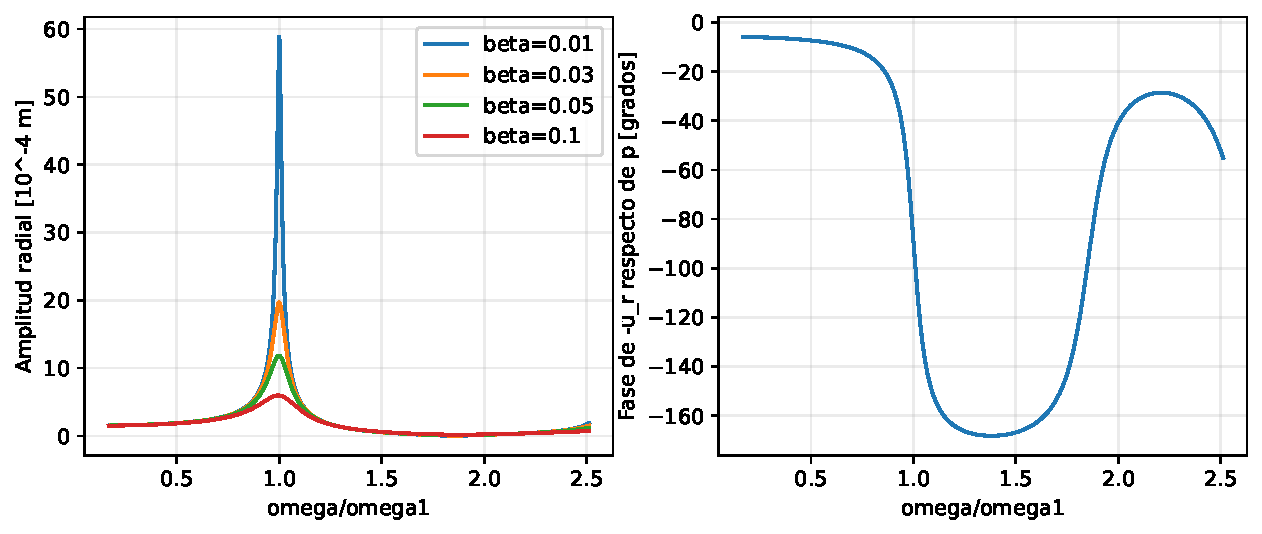
\includegraphics[width=\textwidth]{amortiguamiento_fase.pdf}
\caption{Soluci\'on anal\'itica: efecto del amortiguamiento sobre la
amplitud y fase de la respuesta hacia adentro, $-u_r$, para $\beta=0.05$
en el panel derecho. La fase depende de la convenci\'on temporal y del
signo elegido para medir el desplazamiento.}
\label{fig:amortiguamiento}
\end{figure}

\section{El campo en el interior}
La expresi\'on \eqref{eq:ur-A} permite calcular el desplazamiento en
cualquier radio. La figura~\ref{fig:interior} muestra amplitudes e
instant\'aneas reales; no son la misma cantidad. En $r=0$, el
desplazamiento es cero por regularidad y simetr\'ia.

\begin{figure}[htbp]
\centering
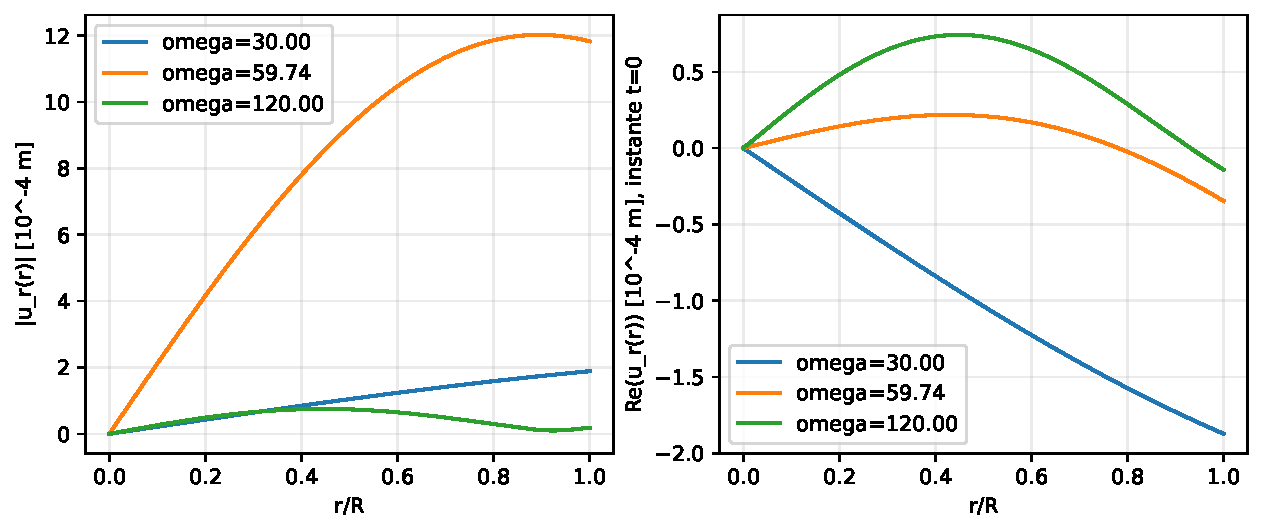
\includegraphics[width=\textwidth]{campo_interior_analitico.pdf}
\caption{Campo interior calculado exclusivamente con la soluci\'on
anal\'itica. Izquierda: amplitud. Derecha: desplazamiento real en $t=0$.
El notebook no implementa una evaluaci\'on BEM interior en su m\'etodo
\code{resolver}.}
\label{fig:interior}
\end{figure}

\chapter{La soluci\'on fundamental: construir las influencias}
\label{ch:fundamental}

\section{Por qu\'e aparece una fuerza puntual auxiliar}
El BEM utiliza la respuesta de un medio homog\'eneo infinito a una
fuerza concentrada. Esta respuesta no satisface por s\'i sola la presi\'on
del cilindro; es una pieza elemental con la que se representa el campo.
Como en circuitos se utiliza la respuesta a un impulso, aqu\'i se utiliza
la respuesta a una fuerza elemental.

En un modelo bidimensional, la fuente puntual en la secci\'on representa
una fuerza por unidad de longitud axial en el modelo tridimensional.
No se debe sustituir la soluci\'on fundamental 3D, que tiene otra
dependencia con la distancia.

\section{Dos puntos y una convenci\'on de \'indices}
Distinguimos:
\begin{equation}
 \vect\xi=\text{punto fuente},\quad
 \vect x=\text{punto de integraci\'on},\quad
 d=|\vect x-\vect\xi|,\quad
 e_j=\frac{x_j-\xi_j}{d}.
 \label{eq:distancia}
\end{equation}
En este cap\'itulo usamos $d$ para no confundir la distancia entre
puntos con el radio $r$ del cilindro. El c\'odigo llama \code{r} a $d$
y \code{ri} a las componentes $e_j$.

Se adopta la convenci\'on del notebook:
\begin{equation}
 U_{ij}=\text{desplazamiento en direcci\'on }j
 \text{ debido a una fuerza unitaria en direcci\'on }i.
\end{equation}
$T_{ij}$ es la componente $j$ de la tracci\'on de ese mismo estado
auxiliar, usando la normal en $\vect x$. En la ecuaci\'on integral,
$i$ identifica la ecuaci\'on y $j$ la componente del dato que se integra.
Aunque $U$ es sim\'etrico, no se debe transponer $T$ por analog\'ia.

\section{Del operador el\'astico a dos funciones de Helmholtz}
Los potenciales longitudinal y transversal satisfacen ecuaciones de
Helmholtz con
\begin{equation}
 k_s=\omega/c_s,\qquad k_p=\omega/c_p.
\end{equation}
Para la convenci\'on $e^{+\ii\omega t}$, una funci\'on fundamental escalar
saliente se escribe
\begin{equation}
 g_\alpha(d)=\frac{1}{2\pi}K_0(\ii k_\alpha d),\qquad
 (\nabla^2+k_\alpha^2)g_\alpha=-\delta(\vect x-\vect\xi),
 \quad \alpha=s,p.
 \label{eq:green-escalar}
\end{equation}
$K_n$ es una funci\'on de Bessel modificada de segunda especie.
El argumento es complejo: no significa que la respuesta del problema
ondulatorio se haya sustituido por una respuesta est\'atica evanescente.
Para argumentos reales de onda, esta representaci\'on equivale a usar
una funci\'on de Hankel saliente consistente con $e^{+\ii\omega t}$.

La soluci\'on fundamental el\'astica se construye como
\begin{equation}
 U_{ij}=\frac1\mu\left[
 \delta_{ij}g_s+\frac1{k_s^2}
       \frac{\partial^2(g_s-g_p)}{\partial x_i\partial x_j}\right].
 \label{eq:U-potenciales}
\end{equation}
Para verificar la forma de esta expresi\'on, definamos el operador
$\mathcal L=\mu\nabla^2+(\lambda+\mu)\nabla\nabla\cdot+\rho\omega^2$.
La aplicaci\'on al primer t\'ermino produce una fuente
$-\delta_{ij}\delta$ y una contribuci\'on longitudinal
$[(\lambda+\mu)/\mu]\partial_i\partial_jg_s$.

Si $f=g_s-g_p$, las fuentes escalares se cancelan y
\begin{equation}
 (\nabla^2+k_p^2)f=(k_p^2-k_s^2)g_s.
\end{equation}
Adem\'as, para un gradiente,
$\mathcal L\nabla h=(\lambda+2\mu)\nabla(\nabla^2+k_p^2)h$.
Por tanto, la contribuci\'on del segundo t\'ermino en
\eqref{eq:U-potenciales} es
\begin{equation}
 \frac{\lambda+2\mu}{\mu k_s^2}
       (k_p^2-k_s^2)\partial_i\partial_jg_s
 =-\frac{\lambda+\mu}{\mu}\partial_i\partial_jg_s.
\end{equation}
Se cancelan las contribuciones longitudinales sobrantes y queda la
fuente el\'astica unitaria requerida. Esta comprobaci\'on explica por
qu\'e se necesitan ambas velocidades.

\section{Deducir la forma utilizada por el programa}
Para una funci\'on radial $f(d)$:
\begin{align}
 \partial_i f&=f'e_i,\\
 \partial_i\partial_j f
   &=\left(f''-\frac{f'}d\right)e_ie_j+\frac{f'}d\delta_{ij}.
 \label{eq:hessiano-radial}
\end{align}
Definimos
\begin{equation}
 z_s=\ii\omega d/c_s,\quad z_p=\ii\omega d/c_p,\quad
 \gamma=c_s/c_p,\quad z_p=\gamma z_s.
\end{equation}
Con $K_0'(z)=-K_1(z)$ y la recurrencia
$K_2(z)=K_0(z)+2K_1(z)/z$, al insertar
\eqref{eq:hessiano-radial} en \eqref{eq:U-potenciales} se obtiene
\begin{equation}
 \boxed{U_{ij}=\frac{1}{2\pi\mu}
             \left(\psi\delta_{ij}-\chi e_ie_j\right),}
 \label{eq:U-final}
\end{equation}
donde
\begin{align}
 \psi&=K_0(z_s)+\frac{K_1(z_s)-\gamma K_1(z_p)}{z_s},\\
 \chi&=K_2(z_s)-\gamma^2K_2(z_p).
 \label{eq:psi-chi}
\end{align}
Una forma de seguir el \'algebra es observar que el coeficiente de
$\delta_{ij}$ contiene
\begin{equation}
 g_s+\frac{f'}{k_s^2d}
 =\frac{1}{2\pi}\left[
 K_0(z_s)+\frac{K_1(z_s)-\gamma K_1(z_p)}{z_s}\right],
\end{equation}
y el de $e_ie_j$ es
\begin{equation}
 \frac{f''-f'/d}{k_s^2}
 =-\frac{K_2(z_s)-\gamma^2K_2(z_p)}{2\pi}.
\end{equation}

\section{Derivadas radiales calculadas por \texttt{psi\_chi}}
Sean $a_s=\ii\omega/c_s$ y $a_p=\ii\omega/c_p$.
Aplicando regla del producto y de la cadena:
\begin{align}
 \psi'={}&a_sK_0'(z_s)
  +\frac{a_sK_1'(z_s)-\gamma a_pK_1'(z_p)}{z_s}
  -\frac{a_s[K_1(z_s)-\gamma K_1(z_p)]}{z_s^2},\\
 \chi'={}&a_sK_2'(z_s)-\gamma^2a_pK_2'(z_p).
 \label{eq:derivadas-kernels}
\end{align}
En SciPy, \code{kv(n,z)} eval\'ua $K_n(z)$ y
\code{kvp(n,z)} su derivada respecto a $z$, no respecto a $d$.
Por eso el c\'odigo multiplica por \code{dzs} o \code{dzp}.

\chapter{De la soluci\'on fundamental a su tracci\'on}
\label{ch:traccion}

\section{Derivar primero el desplazamiento}
Las identidades geom\'etricas necesarias son
\begin{equation}
 \frac{\partial d}{\partial x_k}=e_k,\qquad
 \frac{\partial e_i}{\partial x_k}
       =\frac{\delta_{ik}-e_ie_k}{d}.
\end{equation}
Aplic\'andolas a \eqref{eq:U-final}:
\begin{align}
 \partial_kU_{ij}=\frac{1}{2\pi\mu}\bigg[
 &\psi'e_k\delta_{ij}-\chi'e_ke_ie_j\\
 &-\frac{\chi}{d}
   \left(\delta_{ik}e_j+\delta_{jk}e_i-2e_ie_je_k\right)\bigg].
 \label{eq:grad-U}
\end{align}
Esta expresi\'on ya permite calcular deformaciones, esfuerzos y
tracciones del estado auxiliar.

\section{Aplicar Hooke y multiplicar por la normal}
Para una fuerza auxiliar en direcci\'on $i$, el desplazamiento es la
fila $U_{ij}$ y su tracci\'on es
\begin{equation}
 T_{ij}=\lambda n_j\partial_kU_{ik}
      +\mu n_k(\partial_kU_{ij}+\partial_jU_{ik}).
 \label{eq:T-hooke}
\end{equation}
En dos dimensiones, la divergencia de esa fila resulta
\begin{equation}
 \partial_kU_{ik}=\frac{1}{2\pi\mu}
           \left(\psi'-\chi'-\frac{\chi}{d}\right)e_i.
\end{equation}
Definiendo $s=\vect e\cdot\vect n$, las otras dos contracciones son
\begin{align}
 n_k\partial_kU_{ij}
 &=\frac{1}{2\pi\mu}\left[
 \psi's\delta_{ij}-\chi'se_ie_j
 -\frac{\chi}{d}(n_ie_j+n_je_i-2se_ie_j)\right],\\
 n_k\partial_jU_{ik}
 &=\frac{1}{2\pi\mu}\left[
 \psi'e_jn_i-\chi'se_ie_j
 -\frac{\chi}{d}(\delta_{ij}s+n_je_i-2se_ie_j)\right].
\end{align}
Agrupando t\'erminos en \eqref{eq:T-hooke}:
\begin{align}
 \boxed{\begin{aligned}
 T_{ij}=\frac1{2\pi}\bigg[&
 \left(\psi'-\frac{\chi}{d}\right)(\delta_{ij}s+e_jn_i)\\
 &-\frac{2\chi}{d}(e_in_j-2e_ie_js)-2\chi'e_ie_js\\
 &+\frac{\lambda}{\mu}
    \left(\psi'-\chi'-\frac{\chi}{d}\right)e_in_j\bigg].
 \end{aligned}}
 \label{eq:T-final}
\end{align}
Esta f\'ormula explica cada uno de los cuatro grupos de sumandos de
\code{T} dentro de \code{kernels}.

\section{Qu\'e ocurre cerca de la fuente}
Las expansiones de peque\~no argumento contienen
\begin{align}
 K_0(z)&=-\log(z/2)-\gamma_{\rm E}+O(z^2\log z),\\
 K_1(z)&=\frac1z+\frac z2
          [\log(z/2)+\gamma_{\rm E}-1/2]+O(z^3\log z),\\
 K_2(z)&=\frac2{z^2}-\frac12+O(z^2\log z).
 \label{eq:K-asintoticas}
\end{align}
$\gamma_{\rm E}$ es la constante de Euler; no es la relaci\'on de
velocidades $\gamma$.
Como $z_p=\gamma z_s$, los t\'erminos $1/z_s^2$ de $\chi$ se cancelan:
\begin{equation}
  \chi=\frac{\gamma^2-1}{2}+O(d^2\log d).
  \label{eq:chi-limite}
\end{equation}
Adem\'as,
\begin{equation}
 \psi=-\frac{1+\gamma^2}{2}\log d+C(\omega)
       +O(d^2\log d).
\end{equation}
La relaci\'on el\'astica
\begin{equation}
 \gamma^2=\frac{\mu}{\lambda+2\mu}
          =\frac{1-2\nu}{2(1-\nu)}
\end{equation}
permite recuperar la parte espacial singular de Kelvin:
\begin{equation}
 U^s_{ij}=\frac{1}{8\pi\mu(1-\nu)}
 \left[-(3-4\nu)\log(d/d_0)\delta_{ij}+e_ie_j\right].
 \label{eq:kelvin-U}
\end{equation}
La longitud de referencia $d_0$ solo fija una constante en el logaritmo.
El n\'ucleo din\'amico puede diferir en una constante isot\'ropa
dependiente de la frecuencia; no se debe afirmar que todo $U$ tiene un
l\'imite est\'atico finito en 2D al hacer $\omega\to0$.

\section{N\'ucleo de tracci\'on est\'atico}
Derivando \eqref{eq:kelvin-U} y aplicando
\eqref{eq:T-hooke} se obtiene
\begin{equation}
 \boxed{T^s_{ij}=
 -\frac{1}{4\pi(1-\nu)d}
 \left[s\big((1-2\nu)\delta_{ij}+2e_ie_j\big)
       -(1-2\nu)(e_in_j-e_jn_i)\right].}
 \label{eq:kelvin-T}
\end{equation}
El ap\'endice~\ref{app:kelvin} desarrolla esa simplificaci\'on.
Lo esencial para la integraci\'on es
\begin{equation}
 U=O(\log d),\quad T=O(1/d),\quad
 T-T^s=O(d\log d)
 \quad\text{para frecuencia fija y }d\to0.
 \label{eq:ordenes}
\end{equation}
La diferencia pierde la singularidad $1/d$, aunque su c\'alculo por
resta directa puede ser delicado en aritm\'etica finita.

\begin{figure}[htbp]
\centering
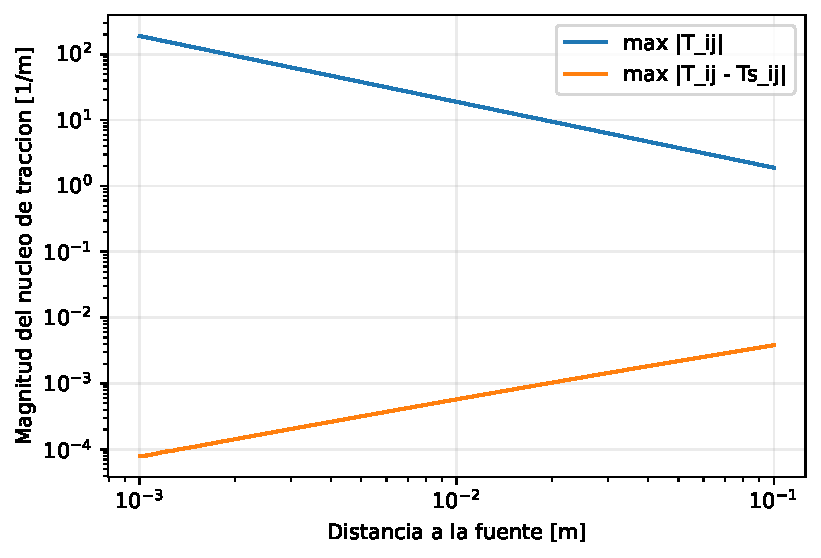
\includegraphics[width=0.76\textwidth]{regularizacion.pdf}
\caption{Evaluaci\'on de los n\'ucleos a $\omega=40$ rad/s a lo largo
de una direcci\'on fija. El n\'ucleo din\'amico crece cerca de la fuente,
mientras que la diferencia con Kelvin disminuye en el intervalo mostrado.
No se incluyen distancias extremadamente peque\~nas, donde la resta
directa pierde precisi\'on.}
\label{fig:regularizacion}
\end{figure}

\chapter{La identidad integral de contorno}
\label{ch:integral}

\section{Reciprocidad: comparar dos estados del mismo material}
Sean un estado real $(\vect u,\vect\sigma)$ y un estado auxiliar
$(\vect v,\vect\tau)$ en el mismo medio. Hooke y la simetr\'ia de los
tensores implican
\begin{equation}
 u_{i,j}\tau_{ij}=v_{i,j}\sigma_{ij}.
\end{equation}
Usando la regla del producto:
\begin{align}
 \partial_j(u_i\tau_{ij}-v_i\sigma_{ij})
 &=u_{i,j}\tau_{ij}-v_{i,j}\sigma_{ij}
       +u_i\tau_{ij,j}-v_i\sigma_{ij,j}\\
 &=u_i\tau_{ij,j}-v_i\sigma_{ij,j}.
\end{align}
Ambos estados tienen la misma frecuencia. El real no tiene fuerza
de volumen; el auxiliar tiene una fuerza unitaria en direcci\'on $a$:
\begin{equation}
 \sigma_{ij,j}=-\rho\omega^2u_i,\qquad
 \tau_{ij,j}=-\rho\omega^2v_i-\delta_{ia}\delta(\vect x-\vect\xi).
\end{equation}
Al sustituir, los t\'erminos de inercia se cancelan:
\begin{equation}
 \partial_j(u_i\tau_{ij}-v_i\sigma_{ij})
              =-u_a(\vect x)\delta(\vect x-\vect\xi).
\end{equation}
Integramos en $\Omega$ y aplicamos la divergencia:
\begin{equation}
 \int_\Gamma(u_i t_i^{\rm aux}-v_i t_i)\dd\Gamma
                 =-u_a(\vect\xi),\qquad \vect\xi\in\Omega.
\end{equation}
Identificando $v_j=U_{aj}$ y $t_j^{\rm aux}=T_{aj}$:
\begin{equation}
 \boxed{u_a(\vect\xi)=
 \int_\Gamma U_{aj}t_j\dd\Gamma-
 \int_\Gamma T_{aj}u_j\dd\Gamma,\qquad\vect\xi\in\Omega.}
 \label{eq:somigliana-interior}
\end{equation}
Es la representaci\'on de Somigliana. El interior queda descrito mediante
desplazamientos y tracciones de su frontera.

\begin{cuidado}
Esta reciprocidad utiliza productos bilineales, sin conjugaci\'on compleja.
Conjugarlos cambiar\'ia el operador material y no reproduce la identidad
usada en el notebook. Tener matrices complejas tampoco significa que sean
herm\'iticas.
\end{cuidado}

\section{Llevar el punto fuente a la frontera}
Para obtener ecuaciones sobre los valores del borde, aproximamos
$\vect\xi$ a $\Gamma$. Una peque\~na vecindad alrededor de la fuente
genera un t\'ermino libre:
\begin{equation}
 c_{ij}(\vect\xi)u_j(\vect\xi)+
 \VP\int_\Gamma T_{ij}(\vect x,\vect\xi)u_j(\vect x)\dd\Gamma
 =
 \int_\Gamma U_{ij}(\vect x,\vect\xi)t_j(\vect x)\dd\Gamma.
 \label{eq:BIE}
\end{equation}
En un punto de contorno suave $c_{ij}=\delta_{ij}/2$.
Una forma de entender el factor $1/2$ es que, localmente, el dominio
ocupa media vecindad de una fuente situada en una frontera suave.
La definici\'on rigurosa incluye el l\'imite de la peque\~na superficie
que excluye la singularidad.

El valor principal de Cauchy, indicado por VP, prescribe una manera
consistente de tomar el l\'imite excluyendo la fuente. No equivale a
poner a cero el valor del n\'ucleo en ese punto.

En esquinas, $c_{ij}$ depende de la geometr\'ia y del problema el\'astico:
no debe reemplazarse sin justificaci\'on por $I/2$. El procedimiento
est\'atico del notebook evita calcularlo expl\'icitamente.

\section{Por qu\'e disminuye la dimensi\'on}
La ecuaci\'on diferencial vive en un \'area; la integral vive en su curva
de contorno. El BEM reduce en uno la dimensi\'on de la discretizaci\'on.
Esta ventaja se obtiene a cambio de matrices densas e integrales singulares.
La representaci\'on utilizada presupone material homog\'eneo por dominio
y ausencia de fuerzas de volumen no tratadas por otros procedimientos.

\begin{figure}[htbp]
\centering
\begin{tikzpicture}[>=Stealth,scale=0.9]
 \draw[thick] (0,0) rectangle (4,3);
 \foreach \x in {0.5,1,...,3.5}{\draw[gray!60] (\x,0)--(\x,3);}
 \foreach \y in {0.5,1,...,2.5}{\draw[gray!60] (0,\y)--(4,\y);}
 \node at (2,-0.5){Malla del \'area (tipo FEM)};
 \draw[->,thick] (4.5,1.5)--node[above]{ecuaci\'on integral}(7,1.5);
 \draw[thick] (7.5,0) rectangle (11.5,3);
 \foreach \x in {7.5,8,...,11.5}{
   \fill (\x,0) circle(1.7pt); \fill (\x,3) circle(1.7pt);}
 \foreach \y in {0.5,1,...,2.5}{
   \fill (7.5,\y) circle(1.7pt); \fill (11.5,\y) circle(1.7pt);}
 \node at (9.5,-0.5){Malla de la frontera (BEM)};
 \node[align=center] at (9.5,1.5){Sin nodos\\interiores};
\end{tikzpicture}
\caption{Reducci\'on dimensional conceptual. El dibujo no representa
los elementos concretos del cilindro.}
\end{figure}

\chapter{Elementos cuadr\'aticos y geometr\'ia}
\label{ch:elementos}

\section{Malla global y conectividad}
Para $N_e$ elementos se crean $N=2N_e$ nodos:
\begin{equation}
 \theta_g=\frac{2\pi g}{N},\qquad
 \vect x_g=R(\cos\theta_g,\sin\theta_g)^{\mathsf T},
 \quad g=0,\ldots,N-1.
\end{equation}
La conectividad del elemento $e$, usando \'indices Python, es
\begin{equation}
 \code{conn[e]}=[2e,\ 2e+1,\ (2e+2)\bmod N].
\end{equation}
El m\'odulo cierra el \'ultimo elemento con el nodo cero. Los extremos se
comparten, pero cada elemento tiene su propio nodo intermedio.
No son $3N_e$ nodos independientes.

\begin{figure}[htbp]
\centering
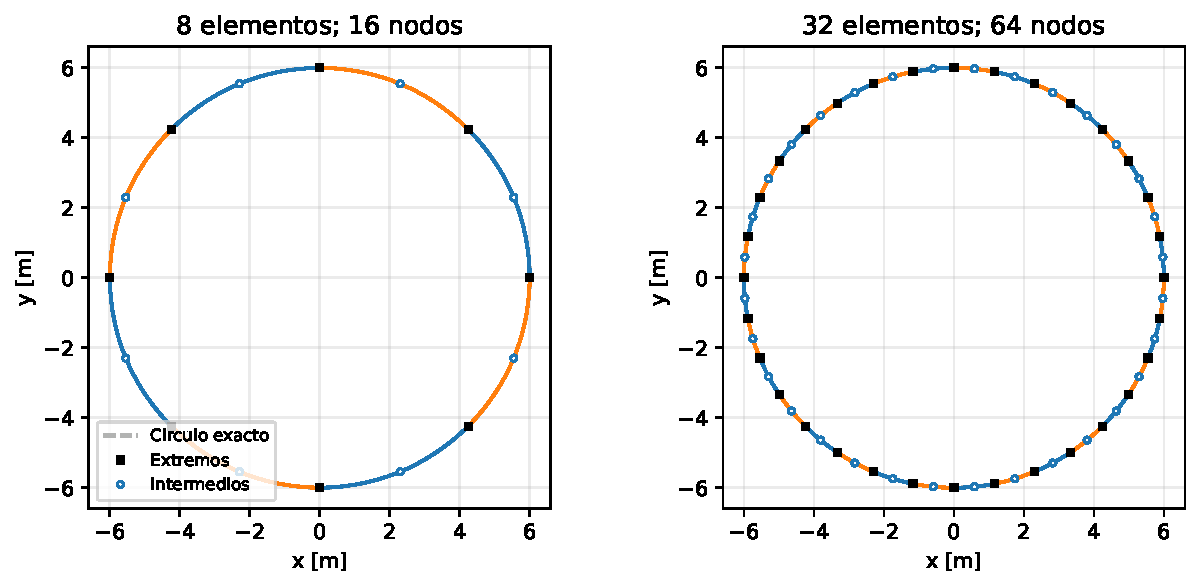
\includegraphics[width=\textwidth]{mallas.pdf}
\caption{Las dos discretizaciones principales. Todos los nodos est\'an
sobre el c\'irculo exacto; las curvas entre nodos son interpolantes
cuadr\'aticos, no arcos circulares exactos.}
\label{fig:mallas}
\end{figure}

\section{Deducir las funciones de forma}
El elemento de referencia tiene nodos
$\eta_1=-1$, $\eta_2=0$, $\eta_3=1$.
Un polinomio de Lagrange que vale uno en el nodo $a$ y cero en los otros es
\begin{equation}
 P_a(\eta)=\prod_{b\ne a}\frac{\eta-\eta_b}{\eta_a-\eta_b}.
\end{equation}
Aplicando la expresi\'on a los tres nodos:
\begin{align}
 P_1&=\frac{(\eta-0)(\eta-1)}{(-1-0)(-1-1)}
       =\frac{\eta(\eta-1)}2,\\
 P_2&=\frac{(\eta+1)(\eta-1)}{(0+1)(0-1)}=1-\eta^2,\\
 P_3&=\frac{(\eta+1)(\eta-0)}{(1+1)(1-0)}
       =\frac{\eta(\eta+1)}2.
\end{align}
Sus derivadas son
\begin{equation}
 P_1'=\eta-\tfrac12,\qquad P_2'=-2\eta,\qquad
 P_3'=\eta+\tfrac12.
\end{equation}
Se verifican las propiedades
\begin{equation}
 P_a(\eta_b)=\delta_{ab},\qquad
 \sum_aP_a=1,\qquad \sum_aP_a'=0.
 \label{eq:particion-unidad}
\end{equation}
La partici\'on de unidad garantiza que un campo constante se interpola
exactamente: es fundamental para el tratamiento de traslaciones r\'igidas.

\begin{figure}[htbp]
\centering
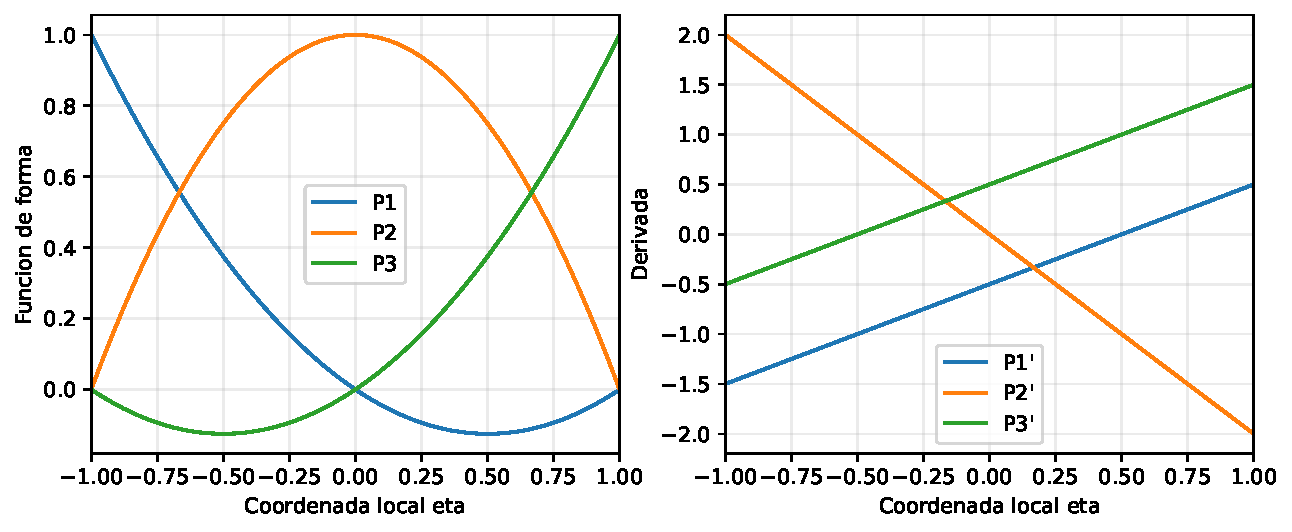
\includegraphics[width=\textwidth]{funciones_forma.pdf}
\caption{Funciones cuadr\'aticas de Lagrange y sus derivadas.
Una funci\'on de forma puede ser negativa entre nodos; esto no invalida
la interpolaci\'on.}
\label{fig:shape}
\end{figure}

\section{Interpolaci\'on isoparam\'etrica}
En el elemento $e$:
\begin{equation}
 \vect x(\eta)=\sum_{a=1}^3P_a(\eta)\vect x_{g(e,a)},\quad
 \vect u(\eta)=\sum_aP_a(\eta)\vect u_{g(e,a)},\quad
 \vect t(\eta)=\sum_aP_a(\eta)\vect t_{g(e,a)}.
 \label{eq:isoparametrico}
\end{equation}
$g(e,a)$ transforma el \'indice local $a$ en uno global.
La misma base describe geometr\'ia y campos: de ah\'i
\emph{isoparam\'etrico}.

\section{Tangente, normal y jacobiano}
La derivada de la geometr\'ia es
\begin{equation}
 \vect x'(\eta)=\sum_aP_a'(\eta)\vect x_{g(e,a)},\qquad
 J(\eta)=\norm{\vect x'(\eta)},\qquad
 \dd\Gamma=J(\eta)\dd\eta.
\end{equation}
$J$ convierte un incremento de coordenada local en longitud f\'isica.
Como la conectividad recorre el c\'irculo en sentido antihorario,
\begin{equation}
 \vect\tau=\frac{(x',y')}{J},\qquad
 \boxed{\vect n=\frac{(y',-x')}{J}.}
 \label{eq:normal}
\end{equation}
Rotar la tangente noventa grados hacia la derecha da la normal exterior.
Invertir el recorrido sin cambiar esta expresi\'on invierte la normal.

\begin{figure}[htbp]
\centering
\begin{tikzpicture}[>=Stealth]
 \draw[thick] (-4,0)--(-1,0);
 \foreach \x/\lab in {-4/-1,-2.5/0,-1/1}{
   \fill (\x,0) circle(2pt);
   \node[below] at (\x,0){$\eta=\lab$};}
 \node at (-2.5,1.3){Referencia};
 \draw[->,thick] (-0.5,0.2)--(1.1,0.2);
 \draw[thick,blue] (1.8,0.5) .. controls (3.4,-1) and (4.6,-1) .. (6,0.2);
 \fill (1.8,0.5) circle(2pt);
 \fill (3.9,-0.55) circle(2pt);
 \fill (6,0.2) circle(2pt);
 \draw[->,green!40!black,thick] (3.9,-0.55)--(5,-0.55)
   node[right]{$\vect\tau$};
 \draw[->,red!70!black,thick] (3.9,-0.55)--(3.9,-1.7)
   node[below]{$\vect n$};
 \node at (3.9,1.3){Elemento f\'isico};
\end{tikzpicture}
\caption{Mapeo de referencia, tangente y normal exterior en un tramo
inferior recorrido de izquierda a derecha. Esquema conceptual.}
\end{figure}

\section{Una sutileza: normal nodal y normal geom\'etrica}
Durante la integraci\'on se usa la normal de la curva interpolada,
\eqref{eq:normal}. Para imponer la presi\'on y proyectar el resultado,
el notebook usa en los nodos $\vect n_g=\vect x_g/R$, la normal del
c\'irculo exacto.

Por tanto, la tracci\'on interpolada
$\sum_aP_a(-p\vect x_a/R)$ no es exactamente $-p$ por la normal de la
curva aproximada en todos sus puntos. Adem\'as, las tangentes de elementos
cuadr\'aticos vecinos no tienen por qu\'e coincidir exactamente en sus
extremos. Son aproximaciones de discretizaci\'on que disminuyen al refinar;
no debe describirse la geometr\'ia como un c\'irculo exacto entre nodos.

\chapter{Colocaci\'on y formaci\'on del sistema matricial}
\label{ch:sistema}

\section{Imponer la identidad en cada nodo}
La colocaci\'on nodal consiste en elegir sucesivamente
$\vect\xi=\vect x_c$ para cada nodo global $c$ y escribir las dos
componentes de \eqref{eq:BIE}. Sustituyendo \eqref{eq:isoparametrico}:
\begin{align}
 c_{ij}(\vect x_c)u_{c,j}
 &+\sum_{e=1}^{N_e}\sum_{a=1}^3
 \left[\VP\int_{-1}^1T_{ij}(\vect x(\eta),\vect x_c)
               P_a(\eta)J(\eta)\dd\eta\right]u_{g(e,a),j}
 \nonumber\\
 &=\sum_{e=1}^{N_e}\sum_{a=1}^3
 \left[\int_{-1}^1U_{ij}(\vect x(\eta),\vect x_c)
               P_a(\eta)J(\eta)\dd\eta\right]t_{g(e,a),j}.
 \label{eq:colocacion}
\end{align}
Se han sacado fuera de la integral los valores nodales desconocidos,
porque no dependen de $\eta$. Dentro quedan cantidades calculables.

\section{Bloques de dos por dos}
Definamos las contribuciones elementales:
\begin{equation}
 \vect G^e_{ca}=\int_{-1}^1\vect U P_aJ\dd\eta,\qquad
 \vect{\widehat H}^e_{ca}=
           \VP\int_{-1}^1\vect T P_aJ\dd\eta.
\end{equation}
Cada una es una matriz $2\times2$. Se suman en la columna global
$g(e,a)$, porque un nodo compartido recibe contribuciones de sus
elementos vecinos. El t\'ermino libre se incorpora en el bloque diagonal
de $\vect H$:
\begin{equation}
  \boxed{\vect H(\omega)\vect u=\vect G(\omega)\vect t.}
  \label{eq:HG}
\end{equation}
Los vectores se ordenan como
\begin{equation}
 \vect u=(u_{0x},u_{0y},u_{1x},u_{1y},\ldots)^{\mathsf T},
\end{equation}
y de la misma forma para $\vect t$. Con $N$ nodos las matrices miden
$2N\times2N$:
\begin{center}
\begin{tabular}{rrrr}
\toprule
Elementos & Nodos & Inc\'ognitas escalares & Tama\~no de cada matriz\\
\midrule
8 & 16 & 32 & $32\times32$\\
32 & 64 & 128 & $128\times128$\\
\bottomrule
\end{tabular}
\end{center}

\section{Comprobaci\'on dimensional de las matrices}
En 2D, $U$ tiene unidades Pa$^{-1}$ y $T$ unidades m$^{-1}$.
Por tanto, $H$ es adimensional y $G$ tiene unidades m/Pa:
\begin{equation}
 [H u]={\rm m},\qquad [G t]=({\rm m/Pa})({\rm Pa})={\rm m}.
\end{equation}
El t\'ermino libre es igualmente adimensional.

\section{Por qu\'e las matrices son densas}
Un elemento lejano sigue influyendo en el punto de colocaci\'on.
En contraste con una matriz de rigidez local de FEM, la mayor\'ia de
los bloques no son cero.
El almacenamiento de matrices escala como $O(N^2)$; una soluci\'on densa
directa suele costar $O(N^3)$. Con cuadratura fija, el ensamblaje tambi\'en
crece aproximadamente con el n\'umero de pares nodo--elemento.
El prec\'alculo detallado del notebook almacena adem\'as datos por par,
no solo por elemento.

\begin{figure}[htbp]
\centering
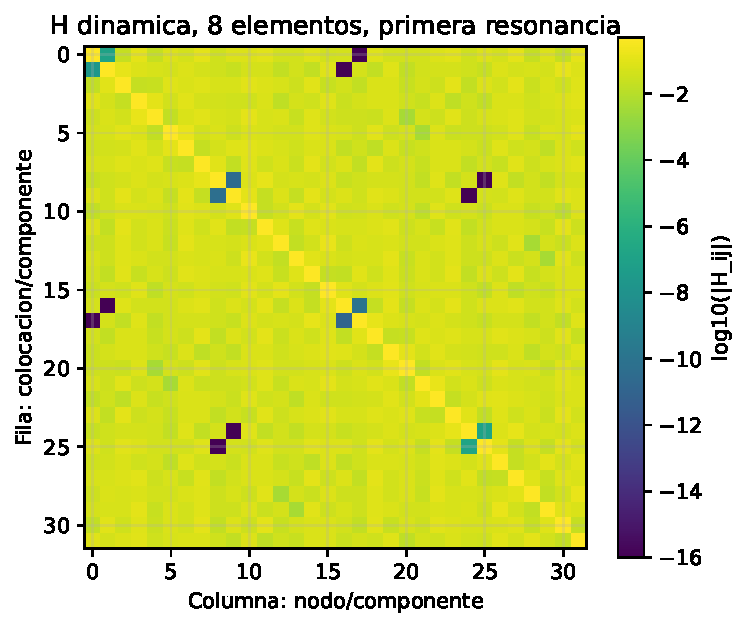
\includegraphics[width=0.72\textwidth]{matriz_h.pdf}
\caption{Magnitud de las entradas de $H$ a la frecuencia de referencia
$\omega_1$. La matriz contiene acoplamiento entre nodos y entre componentes.
La escala es logar\'itmica y representa magnitudes, no fases.}
\end{figure}

\chapter{Cuadratura e integrales singulares}
\label{ch:cuadratura}

\section{De una integral a una suma}
Para una funci\'on regular se aproxima
\begin{equation}
 \int_{-1}^1 f(\eta)\dd\eta
       \simeq\sum_{q=1}^{n_q}w_q f(\eta_q).
 \label{eq:gauss}
\end{equation}
Los puntos y pesos de Gauss-Legendre no son uniformes.
Con $n_q$ puntos se integran exactamente polinomios de grado hasta
$2n_q-1$ en aritm\'etica exacta.
Los n\'ucleos BEM no son polinomios; usar 16 puntos no hace exacta
su integral ni garantiza la misma precisi\'on en todas las situaciones.

\section{Detectar si la fuente pertenece al elemento}
El c\'odigo busca si el nodo global de colocaci\'on aparece en la
conectividad del elemento:
\begin{lstlisting}
loc = np.where(cn == ic)[0]
eta_s = [-1.0, 0.0, 1.0][loc[0]] if len(loc) else None
\end{lstlisting}
Si no aparece, utiliza Gauss ordinario. Si aparece, la fuente est\'a
en $\eta_s=-1,0$ o $1$.

\section{Cambio de variable cuadr\'atico}
Se divide el intervalo en $[-1,\eta_s]$ y $[\eta_s,1]$, omitiendo los
subintervalos de longitud cero. En cada intervalo $[a,b]$ se utiliza
$t\in(0,1)$.

Si la singularidad est\'a en el extremo izquierdo:
\begin{equation}
 \eta=a+(b-a)t^2,\qquad
 \frac{\dd\eta}{\dd t}=2(b-a)t.
 \label{eq:mapa-izquierda}
\end{equation}
Si est\'a en el derecho:
\begin{equation}
 \eta=a+(b-a)[1-(1-t)^2],\qquad
 \frac{\dd\eta}{\dd t}=2(b-a)(1-t).
\end{equation}
Los puntos originales de Gauss en $[-1,1]$ se convierten a
$t_q=(\eta_q+1)/2$ con pesos $w_q/2$. El nuevo peso incorpora tambi\'en
la derivada del mapa.

Para una singularidad logar\'itmica, la primera transformaci\'on convierte
el comportamiento $\log|\eta-a|$ en un producto proporcional a
$t\log t$, que tiende a cero. No elimina algebraicamente todo logaritmo
ni convierte necesariamente el integrando en una funci\'on anal\'itica;
lo hace m\'as favorable para la cuadratura.

\begin{figure}[htbp]
\centering
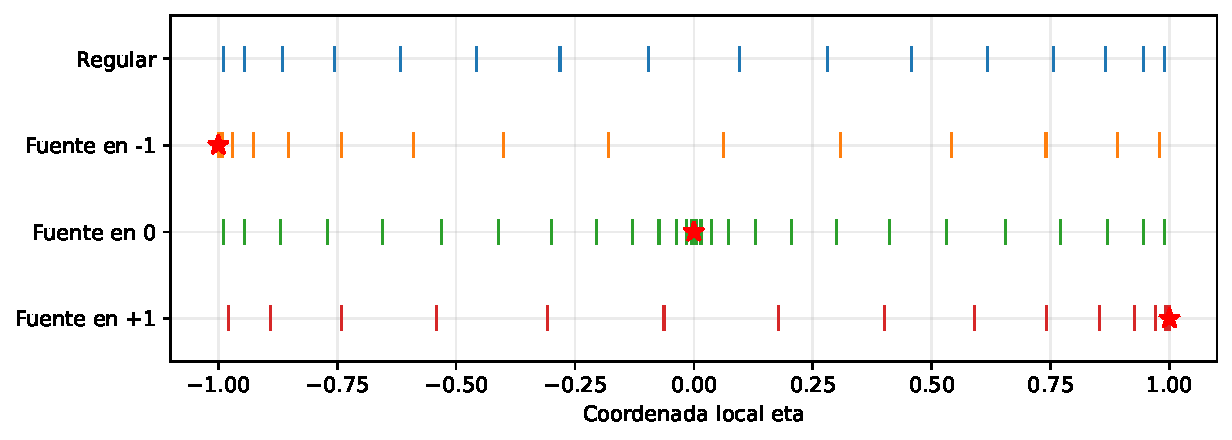
\includegraphics[width=\textwidth]{cuadratura.pdf}
\caption{Puntos realmente utilizados por \code{puntos_cuadratura}.
Una fuente en el nodo intermedio genera dos subintervalos con 16 puntos
cada uno; en un extremo queda un solo subintervalo de 16 puntos.
Los puntos de Gauss nunca coinciden con la estrella roja.}
\label{fig:cuadratura}
\end{figure}

\section{Por qu\'e no basta con evitar evaluar en la fuente}
No calcular $T$ exactamente en $d=0$ evita una divisi\'on literal por
cero, pero no resuelve el valor principal. Una suma de Gauss ordinaria
puede producir un n\'umero finito y, aun as\'i, ser una aproximaci\'on
incorrecta de la integral fuertemente singular.

El notebook combina el cambio de variable con una regularizaci\'on
est\'atica:
\begin{equation}
  T=T^s+(T-T^s).
\end{equation}
La diferencia se integra num\'ericamente. La diagonal de la parte
est\'atica se obtiene con una identidad de movimiento r\'igido.

\section{Derivaci\'on de la identidad de traslaci\'on r\'igida}
Consideremos \emph{el problema est\'atico auxiliar}, no el din\'amico,
con desplazamiento constante $\vect u=\vect a$.
Sus derivadas son cero, luego sus deformaciones, esfuerzos y tracciones
tambi\'en son cero.
Al sustituirlo en la ecuaci\'on integral est\'atica:
\begin{equation}
 \left[\vect c_c+\VP\int_\Gamma\vect T^s\dd\Gamma\right]\vect a=\vect0.
\end{equation}
Como $\vect a$ puede ser cualquier vector constante y
$\sum_aP_a=1$, en forma discreta:
\begin{equation}
  \sum_g\vect H^s_{cg}=\vect0,\qquad
  \boxed{\vect H^s_{cc}=-\sum_{g\ne c}\vect H^s_{cg}.}
  \label{eq:rigido}
\end{equation}
Esta es una suma de \emph{bloques} $2\times2$, no la suma de todas
las entradas escalares de una fila.

Para los bloques $g\ne c$, si el elemento contiene la fuente,
la funci\'on de forma asociada al nodo $g$ se anula en ella.
Su cero compensa el comportamiento $1/d$ y permite integrar esas
contribuciones. Se construyen primero todos los bloques no diagonales;
luego se calcula la diagonal con \eqref{eq:rigido}.

\section{Reconstruir la matriz din\'amica}
La matriz completa se forma como
\begin{equation}
 \boxed{\vect H(\omega)=\vect H^s+
  \int_\Gamma[\vect T(\omega)-\vect T^s]\vect P\dd\Gamma,}
 \label{eq:H-regularizada}
\end{equation}
donde la expresi\'on integral representa el ensamblaje por bloques y
$\vect P$ la interpolaci\'on de las dos componentes.
En forma local:
\begin{equation}
 \Delta\vect H^e_{ca}=
   \int_{-1}^1(\vect T-\vect T^s)P_aJ\dd\eta.
\end{equation}
Se incluyen todos los nodos, tambi\'en $g=c$, en esta correcci\'on.

\begin{cuidado}[No sumar el t\'ermino libre dos veces]
La diagonal construida con movimiento r\'igido ya incluye
$c_{ij}$ m\'as el valor principal est\'atico. No se debe a\~nadir
otro $I/2$ despu\'es de aplicar \eqref{eq:rigido}.
Tampoco debe imponerse suma de bloques cero a la matriz din\'amica:
una traslaci\'on arm\'onica tiene aceleraci\'on y no es una soluci\'on
libre de fuerzas de volumen a frecuencia no nula.
\end{cuidado}

\chapter{Lectura guiada de la implementaci\'on}
\label{ch:codigo}

\section{Mapa de funciones}
\begin{longtable}{p{0.28\textwidth}p{0.65\textwidth}}
\toprule
Nombre & Responsabilidad\\
\midrule
\endhead
\code{material} & M\'odulos complejos y velocidades de onda.\\
\code{u_r_analitico} & Referencia exacta del desplazamiento radial superficial.\\
\code{shape}, \code{dshape} & Funciones cuadr\'aticas y sus derivadas.\\
\code{malla_circulo} & Nodos y conectividad antihoraria.\\
\code{puntos_cuadratura} & Gauss ordinario o partici\'on y mapeo cuadr\'atico.\\
\code{psi_chi} & Funciones radiales de los n\'ucleos y sus derivadas.\\
\code{kernels} & Tensores din\'amicos $U_{ij}$ y $T_{ij}$.\\
\code{kernel_Ts} & Tracci\'on de Kelvin en deformaci\'on plana.\\
\code{BEMCilindro.__init__} & Geometr\'ia de integraci\'on y matriz est\'atica.\\
\code{BEMCilindro.matrices} & Ensamblaje din\'amico de $H$ y $G$.\\
\code{BEMCilindro.resolver} & Aplicar presi\'on, resolver y proyectar radialmente.\\
\bottomrule
\caption{Correspondencia entre el modelo matem\'atico y el notebook.}
\end{longtable}

\section{Constructor: preparar lo que no cambia con la frecuencia}
Al ejecutar
\begin{lstlisting}
bem8 = BEMCilindro(R, 8, mat)
\end{lstlisting}
el constructor guarda la geometr\'ia y recorre cada par
(nodo de colocaci\'on, elemento). El prec\'alculo depende de ambos:
el tratamiento de cuadratura cambia si ese elemento contiene la fuente.

\begin{lstlisting}
Pn, dP = shape(eta), dshape(eta)
X, dX = Pn @ self.nodes[cn], dP @ self.nodes[cn]
J = np.linalg.norm(dX, axis=-1)
nrm = np.stack([dX[:, 1], -dX[:, 0]], -1)/J[:, None]
W = Pn*(J*wq)[:, None]
Ts = kernel_Ts(X, xi, nrm, m["nu"])
\end{lstlisting}
Cada instrucci\'on tiene una correspondencia directa:
\begin{align}
 \code{X[q]}&=\vect x(\eta_q),&
 \code{dX[q]}&=\vect x'(\eta_q),\\
 \code{J[q]}&=J(\eta_q),&
 \code{W[q,a]}&=P_a(\eta_q)J(\eta_q)w_q.
\end{align}
Se guardan \code{cn, X, nrm, W, Ts} en \code{self.quad}.
Tambi\'en se construye $\vect H^s$ fuera de la diagonal y se completa
con \eqref{eq:rigido}. La geometr\'ia y $H^s$ no se vuelven a calcular
para cada frecuencia de una misma instancia.

\section{Dimensiones de los arreglos}
\begin{table}[htbp]
\centering
\begin{tabular}{lll}
\toprule
Arreglo & Forma & Significado\\
\midrule
\code{nodes} & $(N,2)$ & Coordenadas globales\\
\code{conn} & $(N_e,3)$ & Conectividad\\
\code{Pn}, \code{dP} & $(n_q,3)$ & Base y derivadas\\
\code{X}, \code{dX}, \code{nrm} & $(n_q,2)$ & Datos geom\'etricos\\
\code{J}, \code{wq} & $(n_q,)$ & Jacobianos y pesos\\
\code{W} & $(n_q,3)$ & Pesos por nodo local\\
\code{U}, \code{T}, \code{Ts} & $(n_q,2,2)$ & N\'ucleos\\
\code{Gb}, \code{Hb} & $(3,2,2)$ & Tres bloques locales\\
\code{H}, \code{G} & $(2N,2N)$ & Matrices globales\\
\bottomrule
\end{tabular}
\caption{Formas de los arreglos. En elementos partidos,
$n_q$ puede ser 32 en vez de 16.}
\end{table}

\section{Entender \texttt{einsum} sin magia}
La instrucci\'on
\begin{lstlisting}
Gb = np.einsum("qa,qij->aij", W, U)
\end{lstlisting}
significa exactamente
\begin{equation}
  \code{Gb[a,i,j]}=\sum_q\code{W[q,a]}\code{U[q,i,j]}.
\end{equation}
El \'indice $q$ no aparece a la derecha de la flecha, as\'i que se suma.
Los \'indices $a,i,j$ sobreviven. Es una forma vectorizada de escribir:
\begin{lstlisting}
Gb = np.zeros((3, 2, 2), dtype=complex)
for a in range(3):
    for i in range(2):
        for j in range(2):
            for q in range(len(W)):
                Gb[a, i, j] += W[q, a]*U[q, i, j]
\end{lstlisting}
Este segundo bloque es explicativo, no un reemplazo propuesto para el
c\'odigo original.

\section{Ensamblar una frecuencia}
El m\'etodo \code{matrices(w)} empieza con
\begin{lstlisting}
G = np.zeros((2*N, 2*N), complex)
H = self.Hs.astype(complex)
\end{lstlisting}
La conversi\'on permite acumular contribuciones complejas sin modificar
la matriz est\'atica guardada. Para cada par nodo--elemento:
\begin{lstlisting}
U, T = kernels(X, xi, nrm, w, self.m)
Gb = np.einsum("qa,qij->aij", W, U)
Hb = np.einsum("qa,qij->aij", W, T - Ts)
for a, g in enumerate(cn):
    G[2*ic:2*ic+2, 2*g:2*g+2] += Gb[a]
    H[2*ic:2*ic+2, 2*g:2*g+2] += Hb[a]
\end{lstlisting}
Las dos filas corresponden a las dos ecuaciones del nodo de colocaci\'on
\code{ic}; las dos columnas, a las componentes del nodo global \code{g}.
El operador \code{+=} es imprescindible: distintas contribuciones llegan
a la misma posici\'on global.

\section{Aplicar la presi\'on y resolver}
\begin{lstlisting}
H, G = self.matrices(w)
nrm = self.nodes/self.R
t = (-p*nrm).ravel()
u = np.linalg.solve(H, G @ t).reshape(-1, 2)
return (u*nrm).sum(-1)
\end{lstlisting}
Interpretaci\'on:
\begin{enumerate}
 \item Obtener las matrices de la frecuencia.
 \item Calcular las normales radiales nodales.
 \item Aplanar las tracciones en el orden $(t_{0x},t_{0y},\ldots)$.
 \item Formar el segundo miembro $\vect b=\vect G\vect t$.
 \item Resolver $\vect H\vect u=\vect b$ con un solucionador lineal.
 \item Reordenar el vector a $N$ filas de dos componentes.
 \item Calcular $u_{r,g}=u_{x,g}n_{x,g}+u_{y,g}n_{y,g}$.
\end{enumerate}
No se forma expl\'icitamente $H^{-1}$: resolver el sistema es preferible
en costo y estabilidad. Tampoco se utiliza conjugaci\'on en la
proyecci\'on radial, porque la normal geom\'etrica es real.

\begin{idea}[Qu\'e devuelve realmente el m\'etodo]
\code{resolver} devuelve $N$ desplazamientos radiales complejos, uno
por nodo. No devuelve directamente la amplitud media ni todo el campo
interior. La instrucci\'on posterior
\code{np.abs(bem.resolver(w)).mean()} calcula el promedio de amplitudes.
En general, $\operatorname{media}|u|$ y
$|\operatorname{media}u|$ son cantidades distintas.
\end{idea}

\section{Algoritmo completo}
\begin{figure}[htbp]
\centering
\begin{tikzpicture}[>=Stealth,node distance=0.45cm,
 box/.style={draw,rounded corners,align=center,text width=11cm,
 minimum height=0.8cm,fill=blue!4}]
 \node[box] (a){Leer $R,\rho,\mu_0,\nu,\beta,p$ y elegir $N_e$};
 \node[box,below=of a] (b){Crear nodos, conectividad y reglas de cuadratura\\
 para cada par colocaci\'on--elemento};
 \node[box,below=of b] (c){Precalcular $X,J,\vect n,W,T^s$ y construir $H^s$\\
 con la identidad de traslaci\'on r\'igida};
 \node[box,below=of c,fill=orange!8] (d){Para cada frecuencia $\omega$:
 evaluar $U,T$ y ensamblar $G$ y $H^s+\Delta H$};
 \node[box,below=of d,fill=orange!8] (e){Construir
 $\vect t=-p\vect n$ y resolver $H\vect u=G\vect t$};
 \node[box,below=of e,fill=orange!8] (f){Proyectar
 $u_r=\vect u\cdot\vect n$ y guardar amplitud, fase y errores};
 \node[box,below=of f] (g){Comparar con la referencia anal\'itica\\
 y repetir con otra malla o cuadratura};
 \foreach \s/\t in {a/b,b/c,c/d,d/e,e/f,f/g}
   \draw[->] (\s)--(\t);
\end{tikzpicture}
\caption{Separaci\'on entre preparaci\'on geom\'etrica y operaciones
repetidas para cada frecuencia.}
\end{figure}

\chapter{Verificaci\'on num\'erica y lectura de resultados}
\label{ch:verificacion}

\section{Verificar por capas}
Una curva visualmente parecida no basta. Conviene verificar:
\begin{enumerate}
 \item \textbf{Interpolaci\'on:} propiedades nodales y partici\'on de unidad.
 \item \textbf{Cuadratura:} pesos que integran una constante correctamente
 y puntos que no eval\'uan la fuente.
 \item \textbf{N\'ucleos:} Hooke aplicado a derivadas num\'ericas de $U$
 debe reproducir $T$; $U$ debe satisfacer Navier fuera de la fuente.
 \item \textbf{Regularizaci\'on:} la parte est\'atica debe anular dos
 traslaciones independientes.
 \item \textbf{Sistema lineal:} residuo algebraico peque\~no.
 \item \textbf{Soluci\'on f\'isica:} comparaci\'on de amplitud, fase,
 simetr\'ia y componente tangencial con la referencia.
\end{enumerate}
El script adjunto comprueba estas propiedades mediante pruebas
num\'ericas enfocadas y detiene la ejecuci\'on si fallan sus umbrales.
No sustituye una demostraci\'on general de convergencia.

\section{Comprobar el n\'ucleo de tracci\'on}
Para un paso $h$:
\begin{equation}
 \partial_kU_{ij}(\vect x)\simeq
 \frac{U_{ij}(\vect x+h\vect e_k)-U_{ij}(\vect x-h\vect e_k)}{2h}.
\end{equation}
Se construye la deformaci\'on, se aplica Hooke y se multiplica por
la normal. En el punto de prueba del notebook, con $h=10^{-6}$ m,
el error relativo m\'aximo es aproximadamente
$3.12\times10^{-9}$.

Con segundas diferencias, el residuo relativo de Navier fuera de la
fuente es aproximadamente $4.59\times10^{-6}$ para el paso elegido.
Estos errores incluyen truncamiento y redondeo de las diferencias
finitas: no son directamente el error del solucionador BEM.

\section{Definir el error que se est\'a reportando}
La cantidad del gr\'afico original es
\begin{equation}
 A_h=\frac1N\sum_g|u_{r,g}^{h}|,\qquad
 e_A=\frac{|A_h-|u_r^{\rm an}||}{|u_r^{\rm an}|}.
 \label{eq:error-amplitud}
\end{equation}
Es un error de amplitud \emph{promedio}. No mide por s\'i solo la
precisi\'on de cada nodo ni la fase.

Una verificaci\'on adicional del campo complejo radial es
\begin{equation}
 e_{\mathbb C}=
 \frac{\left(\frac1N\sum_g|u_{r,g}^{h}-u_r^{\rm an}|^2\right)^{1/2}}
 {|u_r^{\rm an}|}.
 \label{eq:error-complejo}
\end{equation}
Para la simetr\'ia tangencial, con
$\vect\tau_g=(-n_{y,g},n_{x,g})$:
\begin{equation}
 e_\theta=
 \frac{\left(\frac1N\sum_g|\vect u_g^h\cdot\vect\tau_g|^2\right)^{1/2}}
 {|u_r^{\rm an}|}.
\end{equation}
La soluci\'on exacta tiene $u_\theta=0$.
Estas medidas se normalizan por una referencia que no sea cero.
Cerca de una antirresonancia no amortiguada conviene usar adem\'as
errores absolutos o una escala fija.

\section{Resultados en frecuencias seleccionadas}
\begin{table}[htbp]
\centering\small
\resizebox{\textwidth}{!}{\begin{tabular}{rrrrrr}
\toprule
$\omega$ & $|u_r^{\rm an}|$ [m] & BEM 8 [m] & $e_{A,8}$ & BEM 32 [m] & $e_{A,32}$\\
\midrule
10.00 & 1.52673e-04 & 1.52622e-04 & 3.33e-04 & 1.52673e-04 & 9.74e-07\\
40.00 & 2.43334e-04 & 2.43094e-04 & 9.84e-04 & 2.43333e-04 & 2.69e-06\\
59.74 & 1.18303e-03 & 1.18059e-03 & 2.06e-03 & 1.18301e-03 & 1.17e-05\\
100.00 & 2.44867e-05 & 2.45248e-05 & 1.55e-03 & 2.44866e-05 & 3.58e-06\\
150.00 & 1.17206e-04 & 1.17275e-04 & 5.93e-04 & 1.17204e-04 & 1.40e-05\\
\bottomrule
\end{tabular}
}
\caption{Amplitudes y error relativo de su promedio. La frecuencia se
expresa en rad/s. La notaci\'on \texttt{e-04} significa
$\times10^{-4}$; los errores son fracciones, no porcentajes.}
\label{tab:verificacion}
\end{table}

Por ejemplo, en $\omega_1$:
\begin{itemize}
 \item Referencia: $1.18303\times10^{-3}$ m.
 \item BEM 8: error de amplitud promedio cercano a $0.206\,\%$.
 \item BEM 32: error de amplitud promedio cercano a $0.00117\,\%$.
\end{itemize}
La conversi\'on a porcentaje multiplica el error relativo por cien.

\begin{table}[htbp]
\centering
\begin{tabular}{rrrrr}
\toprule
$\omega$ & $e_{\mathbb C,8}$ & $e_{\mathbb C,32}$ & $e_{\theta,8}$ & $e_{\theta,32}$\\
\midrule
10.00 & 3.512e-04 & 1.948e-04 & 1.685e-04 & 5.850e-04\\
40.00 & 1.002e-03 & 1.094e-05 & 1.326e-06 & 3.014e-05\\
59.74 & 8.445e-03 & 3.742e-05 & 7.932e-07 & 1.127e-05\\
100.00 & 1.850e-03 & 1.297e-05 & 1.239e-07 & 6.364e-06\\
150.00 & 1.151e-02 & 3.269e-05 & 6.224e-08 & 2.054e-06\\
\bottomrule
\end{tabular}

\caption{Errores RMS del campo complejo radial y del componente
tangencial. Todos son relativos y adimensionales.}
\label{tab:complejo}
\end{table}

La tabla~\ref{tab:complejo} muestra por qu\'e conviene no limitarse a
amplitudes: a $\omega_1$, con 8 elementos,
$e_{\mathbb C}\simeq0.8445\,\%$, mayor que el $0.206\,\%$ de $e_A$.
A 150 rad/s, el error complejo es aproximadamente $1.15\,\%$ aunque el
error de amplitud promedio es solo $0.0593\,\%$.

\section{Respuesta frecuencial}
\begin{figure}[htbp]
\centering
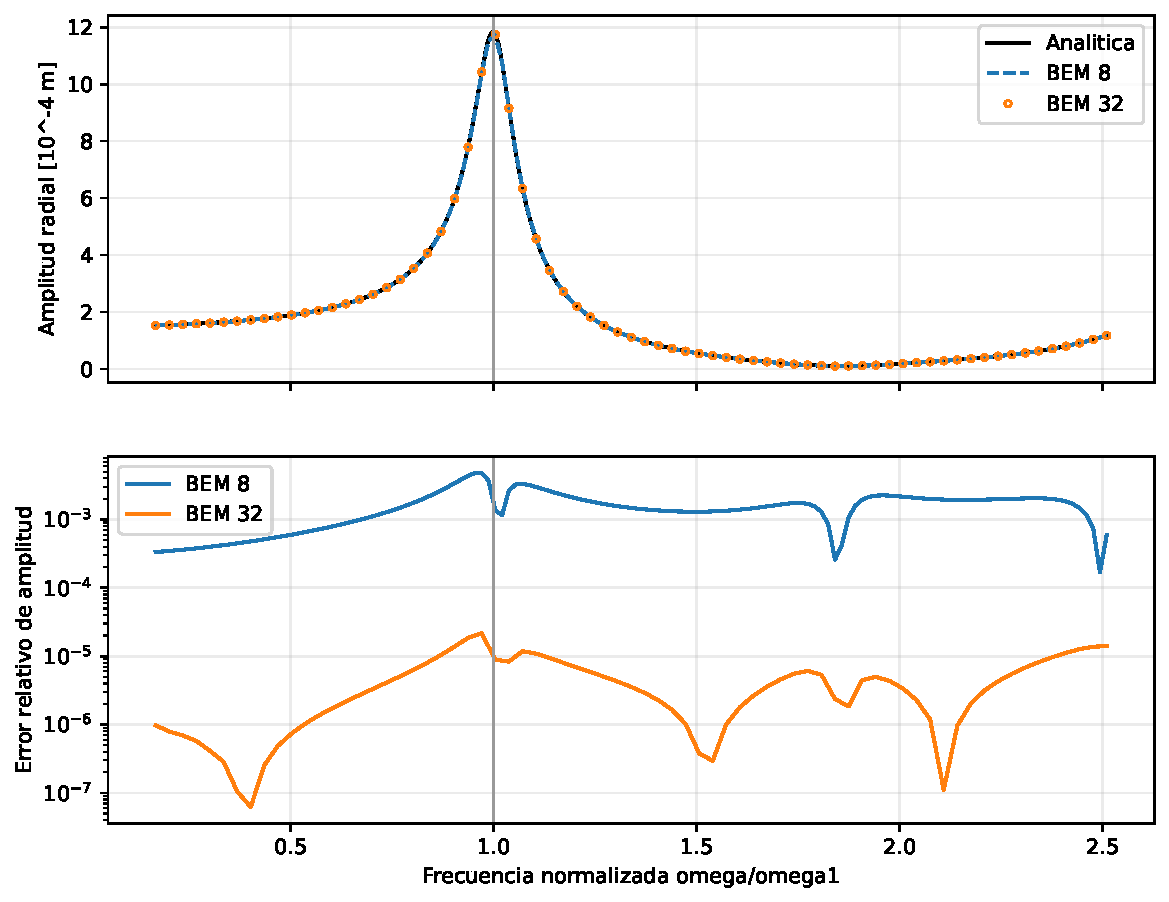
\includegraphics[width=0.95\textwidth]{respuesta_frecuencia.pdf}
\caption{Respuesta del BEM frente a la soluci\'on anal\'itica.
Se utilizan 141 frecuencias para 8 elementos y 71 para 32 elementos,
ambos barridos entre 10 y 150 rad/s. La curva anal\'itica fina tiene
2001 puntos. Estas densidades son las de la gu\'ia; el notebook utiliza
281 y 113 puntos, respectivamente.}
\label{fig:respuesta}
\end{figure}

En los puntos muestreados, el m\'aximo de $e_A$ es aproximadamente
$4.79\times10^{-3}$ para 8 elementos y $2.16\times10^{-5}$ para
32 elementos. Esto equivale a $0.479\,\%$ y $0.00216\,\%$.
Son m\'aximos de barridos discretos, no una cota demostrada para
toda frecuencia del intervalo.

\section{Simetr\'ia y errores nodales}
El modelo anal\'itico impone simetr\'ia axial desde el principio;
el BEM conserva dos componentes por nodo. Por eso es \'util comprobar
que los resultados calculados recuperen esa simetr\'ia.
La malla cuadr\'atica distingue nodos extremos e intermedios y puede
introducir oscilaciones discretas entre ambas familias.

\begin{figure}[htbp]
\centering
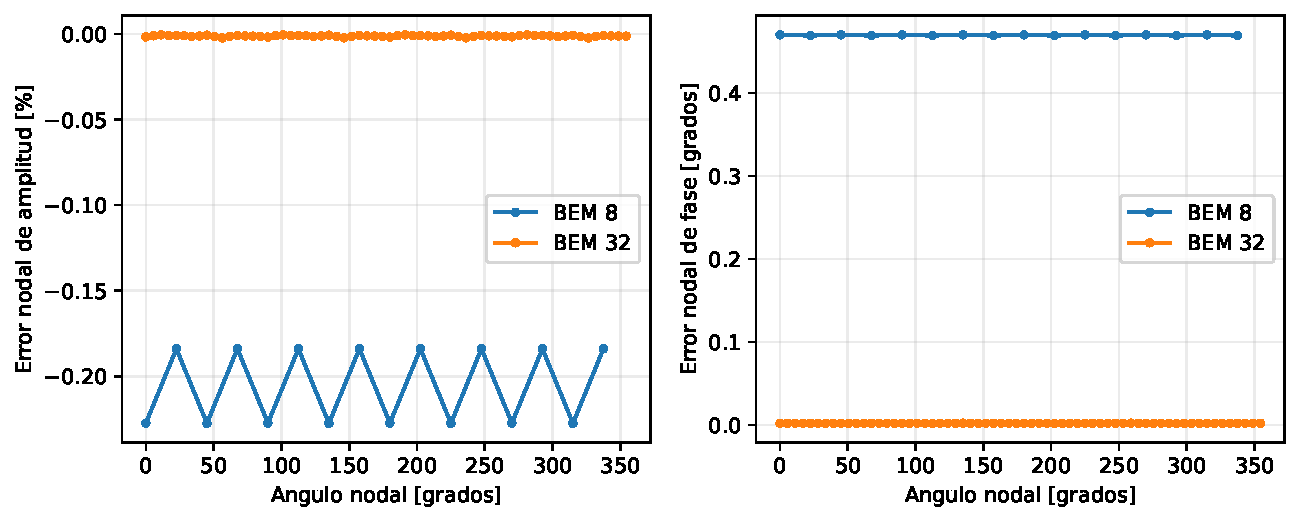
\includegraphics[width=\textwidth]{errores_nodales.pdf}
\caption{Errores nodales en la frecuencia $\omega_1$.
La fase se calcula como $\arg(u_{r,g}^{h}/u_r^{\rm an})$:
cero significa coincidencia de fase. El promedio de amplitudes
puede ocultar variaciones entre nodos.}
\end{figure}

\section{Residuo algebraico y error f\'isico no son lo mismo}
Se mide un residuo hacia atr\'as:
\begin{equation}
 \eta_{\rm alg}=
 \frac{\norm{H\vect u-\vect b}_2}
 {\norm H_F\norm{\vect u}_2+\norm{\vect b}_2},\qquad
 \vect b=G\vect t.
\end{equation}
En las pruebas seleccionadas es del orden de $10^{-17}$.
Esto indica que el sistema \emph{ensamblado} se resuelve con gran
precisi\'on. No demuestra que ese sistema represente exactamente la
geometr\'ia o las integrales continuas.
Un residuo peque\~no puede coexistir con error de malla, de cuadratura
o de evaluaci\'on de n\'ucleos.

\chapter{Convergencia y cancelaci\'on num\'erica}
\label{ch:convergencia}

\section{Refinar la malla}
Sea $h$ una longitud representativa del elemento; en este c\'irculo,
$h\propto1/N_e$. Si una medida de error se comporta como
$e\simeq C h^p$, entonces
\begin{equation}
 e\simeq C' N_e^{-p},\qquad
 p\simeq\frac{\log(e_{N_e}/e_{2N_e})}{\log2}.
 \label{eq:orden}
\end{equation}
El orden observado depende de la regularidad, colocaci\'on, geometr\'ia,
cuadratura y cantidad de salida. No hay que prometer un orden universal
solo porque la interpolaci\'on sea cuadr\'atica.

\begin{figure}[htbp]
\centering
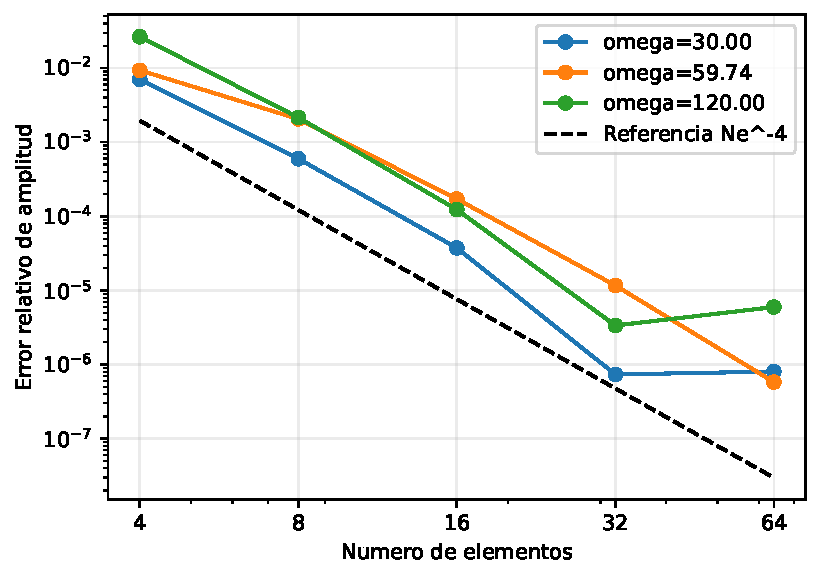
\includegraphics[width=0.8\textwidth]{convergencia.pdf}
\caption{Error de amplitud promedio con 4, 8, 16, 32 y 64 elementos,
manteniendo 16 puntos de Gauss. La recta $N_e^{-4}$ es una referencia
visual, no una garant\'ia. La falta de monoton\'ia indica que la malla
no es la \'unica fuente de error.}
\label{fig:convergencia}
\end{figure}

Por ejemplo, a 30 rad/s el error disminuye desde aproximadamente
$7.02\times10^{-3}$ con cuatro elementos hasta
$7.37\times10^{-7}$ con 32, pero sube ligeramente a
$8.05\times10^{-7}$ con 64.
Un error escalar promedio tambi\'en puede presentar cancelaciones
fortuitas; una pendiente local superior a cuatro no demuestra por
s\'i sola un m\'etodo de orden mayor.

\section{Aumentar puntos de Gauss: comprobar, no suponer}
Se repiti\'o el c\'alculo a 30 rad/s variando la cuadratura, sin cambiar
las f\'ormulas de los n\'ucleos:
\begin{table}[htbp]
\centering
\begin{tabular}{rrr}
\toprule
Puntos de Gauss & $e_A$, 32 elementos & $e_A$, 64 elementos\\
\midrule
12 & 3.200e-06 & 2.762e-06\\
16 & 7.370e-07 & 8.053e-07\\
24 & 2.086e-06 & 2.147e-06\\
32 & 2.647e-05 & 9.783e-04\\
\bottomrule
\end{tabular}

\caption{Sensibilidad real al n\'umero de puntos de Gauss en la
implementaci\'on original. M\'as puntos no siempre mejoran el resultado.}
\label{tab:cuadratura}
\end{table}

\begin{figure}[htbp]
\centering
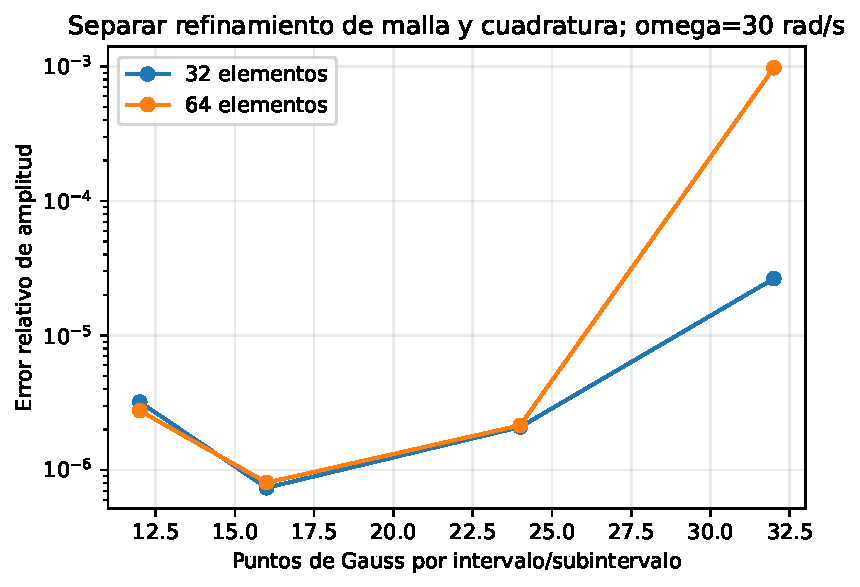
\includegraphics[width=0.78\textwidth]{sensibilidad_cuadratura.pdf}
\caption{Mismo estudio de la tabla~\ref{tab:cuadratura}. La p\'erdida de
precisi\'on al aumentar la cuadratura impide atribuir todo estancamiento
a falta de puntos de integraci\'on.}
\end{figure}

En particular, con 64 elementos y 32 puntos, el error medido se acerca a
$9.78\times10^{-4}$. Esto no significa que la cuadratura de Gauss
empeore matem\'aticamente por tener m\'as puntos; significa que el
algoritmo completo contiene otros efectos num\'ericos.

\section{Por qu\'e restar cantidades grandes puede perder cifras}
Supongamos que deseamos calcular $A-B$, con
$A\simeq B\simeq10^{14}$, pero la diferencia real es del orden de uno.
Errores relativos peque\~nos en $A$ y $B$ pueden ser grandes frente a
su diferencia. Un indicador de sensibilidad de la resta es
\begin{equation}
 \kappa_{\rm resta}\simeq\frac{|A|+|B|}{|A-B|}.
\end{equation}
En $\chi=K_2(z_s)-\gamma^2K_2(z_p)$, cada t\'ermino crece como
$1/d^2$, aunque su diferencia tiende al valor finito de
\eqref{eq:chi-limite}. Las derivadas contienen cancelaciones todav\'ia
m\'as severas.

Para $\nu=0.25$, $\gamma^2=1/3$, por lo que
\begin{equation}
 \lim_{d\to0}\chi=-\frac13,\qquad
 \chi'=O(d\log d)\longrightarrow0.
\end{equation}
Sin embargo, la evaluaci\'on directa en doble precisi\'on produce:

\begin{table}[htbp]
\centering
\begin{tabular}{rrr}
\toprule
$d$ [m] & $\operatorname{Re}\chi$ & $\operatorname{Re}\chi'$ [1/m]\\
\midrule
1e-02 & -0.333339726 & -1.180e-03\\
1e-03 & -0.333333418 & -1.755e-04\\
1e-04 & -0.333333492 & 7.812e-03\\
1e-05 & -0.333282471 & -1.600e+01\\
1e-06 & -0.324218750 & -1.638e+04\\
1e-07 & 0.000000000 & -1.678e+07\\
\bottomrule
\end{tabular}

\caption{Diagn\'ostico de peque\~na distancia a 30 rad/s con el material
del notebook. Los valores extremos de $\chi'$ y la p\'erdida de
$\chi\to-1/3$ evidencian cancelaci\'on y redondeo.}
\label{tab:cancelacion}
\end{table}

El mapeo cuadr\'atico concentra puntos cerca de la fuente.
Al aumentar Gauss, algunos puntos quedan todav\'ia m\'as cerca y
pueden entrar en este r\'egimen problem\'atico.
La tabla verifica directamente una p\'erdida de precisi\'on de los
n\'ucleos a distancias peque\~nas; no descompone cuantitativamente
todo el error de cada integral en una \'unica causa.

\begin{cuidado}[Conclusi\'on pr\'actica]
No es seguro afirmar que cualquier estancamiento desaparece aumentando
Gauss. Una implementaci\'on m\'as robusta puede requerir expansiones
asint\'oticas estables, evaluaci\'on conjunta de diferencias o integraci\'on
singular anal\'itica. Esta gu\'ia identifica y explica la limitaci\'on;
no altera el notebook ni introduce una formulaci\'on nueva.
\end{cuidado}

\section{Separar cuatro errores}
Conviene distinguir conceptualmente:
\begin{enumerate}
 \item \textbf{Modelo:} cilindro infinito, material lineal, deformaci\'on plana.
 \item \textbf{Discretizaci\'on:} geometr\'ia y campos aproximados en elementos.
 \item \textbf{Integraci\'on y n\'ucleos:} cuadratura, singularidades y cancelaci\'on.
 \item \textbf{\'Algebra lineal:} redondeo y condicionamiento del sistema.
\end{enumerate}
No siempre se suman de forma simple: pueden amplificarse o cancelarse.
Para una verificaci\'on seria hay que variar una cosa a la vez y
observar varias medidas de error.

\chapter{L\'imites del modelo y extensiones}
\label{ch:limites}

\section{Frecuencias cercanas a cero}
Un cuerpo libre sometido solo a tracciones admite traslaciones y una
rotaci\'on r\'igida en est\'atica. Esos movimientos no generan
deformaci\'on ni tracci\'on. Por tanto, el problema est\'atico de
Neumann no fija una posici\'on absoluta sin restricciones adicionales.

La presi\'on uniforme satisface equilibrio global:
\begin{equation}
 \int_\Gamma\vect t\dd\Gamma=-p\int_\Gamma\vect n\dd\Gamma=\vect0,
 \qquad
 \int_\Gamma\vect x\times\vect t\dd\Gamma=0.
\end{equation}
Esto hace compatible la carga est\'atica, pero no elimina los movimientos
r\'igidos de la soluci\'on general. La expresi\'on radial anal\'itica
selecciona la soluci\'on sim\'etrica sin esos movimientos.

A frecuencia peque\~na, la matriz din\'amica se aproxima a una matriz
con modos r\'igidos y puede estar mal condicionada. Adem\'as, aparecen
cancelaciones en los argumentos peque\~nos de Bessel. El rango del
notebook comienza en 10 rad/s y no constituye un solucionador est\'atico
general.

\section{Resonancias y amortiguamiento}
El amortiguamiento evita los polos reales ideales de la respuesta.
Aun as\'i, cerca de resonancias puede aumentar la sensibilidad a errores
de par\'ametros o geometr\'ia. El hecho de que una matriz se pueda
resolver no garantiza que el pico est\'e localizado con la precisi\'on
deseada: tambi\'en se debe refinar el muestreo en frecuencia.

\section{Qu\'e no implementa esta clase}
\begin{itemize}
 \item Materiales que var\'ian continuamente dentro del dominio.
 \item Varios dominios o interfaces entre materiales.
 \item Condiciones mixtas de desplazamiento y tracci\'on.
 \item Integraci\'on adaptativa para elementos casi singulares.
 \item Un evaluador BEM del campo interior.
 \item Un algoritmo de inversi\'on ni una red neuronal PINN.
\end{itemize}
Algunas extensiones son posibles con BEM, pero no est\'an presentes
en \code{BEMCilindro}. Por ejemplo, para condiciones mixtas se
reordenan columnas de $H$ y $G$ para reunir los valores desconocidos en
un solo vector. Eso es una ampliaci\'on del problema, no lo que hace
el m\'etodo \code{resolver} actual.

\section{Relaci\'on con problemas inversos}
Este es un \emph{modelo directo}: material, geometr\'ia y carga conocidos
producen desplazamientos. Un problema inverso cambiar\'ia uno o varios
par\'ametros para ajustar observaciones. Antes de usar un modelo directo
dentro de una inversi\'on, debe verificarse: de lo contrario, el algoritmo
puede ajustar errores del modelo en vez de propiedades f\'isicas.

\chapter{Reproducir la gu\'ia y estudiar de forma activa}
\label{ch:reproducir}

\section{Archivos y requisitos}
La carpeta de esta gu\'ia contiene:
\begin{itemize}
 \item \code{guia_bem.tex}: documento principal.
 \item \code{guia_bem.pdf}: versi\'on compilada.
 \item \code{generar_figuras.py}: generaci\'on y comprobaci\'on.
 \item \code{figuras/}: once gr\'aficas vectoriales PDF.
 \item \code{datos/resultados.json}: cifras, errores, estudios y huella
 SHA-256 del notebook utilizado.
 \item \code{datos/tabla_*.tex}: tablas calculadas para el documento.
\end{itemize}
El script requiere Python, NumPy, SciPy y Matplotlib. Para compilar:
una distribuci\'on \LaTeX{} con espa\~nol, TikZ, \code{tcolorbox},
\code{listings} y \code{latexmk}. No se necesita un kernel de Jupyter
para regenerar las figuras.

\section{C\'omo se reutiliza el notebook}
El script lee el JSON del notebook y extrae, mediante el \'arbol de
sintaxis de Python, importaciones, definiciones y asignaciones
seleccionadas de sus celdas conocidas. No ejecuta el barrido completo
ni las celdas de dibujo del notebook.

Las clases y funciones usadas en el c\'alculo son las originales:
no se mantiene una segunda implementaci\'on del BEM. El estudio de
cuadratura cambia temporalmente los arreglos globales de Gauss en la
copia cargada en memoria y los restaura al terminar. No modifica
el archivo original.

Este procedimiento presupone que el notebook local es de confianza.
Si se renombran o eliminan sus identificadores de celda, el script
informa expl\'icitamente el problema; no intenta continuar con datos
inventados.

\section{Comandos}
Desde la ra\'iz del repositorio:
\begin{lstlisting}[language=bash]
OPENBLAS_NUM_THREADS=1 OMP_NUM_THREADS=1 \
  python3 estudio_bignardi/guia_bem/generar_figuras.py

cd estudio_bignardi/guia_bem
latexmk -pdf -interaction=nonstopmode -halt-on-error \
  -outdir=.build guia_bem.tex
cp .build/guia_bem.pdf guia_bem.pdf
\end{lstlisting}
La configuraci\'on de hilos se aplica solo al proceso del comando.
Las figuras se producen con un backend no interactivo y no abren
ventanas. \code{latexmk} repite la compilaci\'on lo necesario para
actualizar referencias, \'indices y numeraci\'on.

\section{Comprobaciones automatizadas}
Entre otras verificaciones, el script exige:
\begin{itemize}
 \item Forma esperada de mallas y propiedades de la interpolaci\'on.
 \item Suma de pesos de cuadratura igual a dos.
 \item Anulaci\'on de dos traslaciones con la matriz est\'atica.
 \item Residuo algebraico hacia atr\'as menor que $10^{-13}$.
 \item Error RMS radial complejo menor que $2\,\%$ en las frecuencias
 seleccionadas de las mallas 8 y 32.
 \item Error de amplitud promedio menor que $1\,\%$ en los barridos
 de ambas mallas.
 \item Error de tracci\'on por diferencias finitas menor que $10^{-6}$
 y residuo relativo de Navier menor que $10^{-3}$ en el punto de prueba.
\end{itemize}
Son umbrales de regresi\'on para este caso, no garant\'ias universales.
Las tablas registran valores medidos, no esos umbrales.

\section{Secuencia sugerida de experimentos}
\begin{enumerate}
 \item Mantener geometr\'ia y material, y duplicar $p$: el desplazamiento
 debe duplicarse por linealidad.
 \item Disminuir $\beta$ sin llegar a cero y observar el pico y la fase.
 \item Comparar nodos extremos e intermedios antes de promediar.
 \item Refinar la malla manteniendo cuadratura fija.
 \item Variar cuadratura con la malla fija y revisar el diagn\'ostico
 de cancelaci\'on, no solo el gr\'afico final.
 \item Comparar amplitud y campo complejo: una buena amplitud no implica
 una buena fase.
\end{enumerate}

\begin{idea}[La cadena conceptual completa]
Desplazamiento $\longrightarrow$ deformaci\'on $\longrightarrow$
esfuerzo $\longrightarrow$ equilibrio din\'amico
$\longrightarrow$ soluci\'on fundamental
$\longrightarrow$ reciprocidad
$\longrightarrow$ identidad integral
$\longrightarrow$ interpolaci\'on y cuadratura
$\longrightarrow H u=G t$
$\longrightarrow$ verificaci\'on frente a una referencia conocida.
\end{idea}

\appendix
\chapter{Funciones de Bessel sin tratarlas como una caja negra}
\label{app:bessel}

\section{Por qu\'e no bastan senos y cosenos}
En una barra recta, una ecuaci\'on como $v''+k^2v=0$ tiene soluciones
senoidales. En coordenadas polares aparecen t\'erminos adicionales:
la longitud de una circunferencia aumenta con el radio y la direcci\'on
radial cambia al recorrerla. Por eso la ecuaci\'on radial
\eqref{eq:ode-radial} contiene $u_r'/r-u_r/r^2$.
Las funciones de Bessel desempe\~nan el papel de senos y cosenos en
esta geometr\'ia, pero con su propia variaci\'on de amplitud.

\section{Construir la soluci\'on regular mediante una serie}
Consideremos la ecuaci\'on de orden general $n$:
\begin{equation}
 s^2v''+sv'+(s^2-n^2)v=0.
\end{equation}
Proponemos una serie de Frobenius
$v(s)=\sum_{m=0}^{\infty}a_m s^{m+\alpha}$.
Al derivar y agrupar potencias:
\begin{equation}
 \sum_{m=0}^{\infty}[(m+\alpha)^2-n^2]a_ms^{m+\alpha}
 +\sum_{m=0}^{\infty}a_ms^{m+\alpha+2}=0.
\end{equation}
El t\'ermino de menor exponente exige
$(\alpha^2-n^2)a_0=0$.
Para la rama regular escogemos $\alpha=n$.
Al igualar el coeficiente de $s^{m+n}$:
\begin{equation}
 m(m+2n)a_m+a_{m-2}=0,\qquad
 a_m=-\frac{a_{m-2}}{m(m+2n)},\quad m\ge2.
\end{equation}
Para $n=0,1$ se obtiene $a_1=0$ y solo quedan potencias de igual
paridad. Escogiendo la normalizaci\'on
$a_0=1/[2^n n!]$, resulta
\begin{equation}
 J_n(s)=\sum_{m=0}^{\infty}
 \frac{(-1)^m}{m!(m+n)!}\left(\frac{s}{2}\right)^{2m+n}.
\end{equation}
En particular:
\begin{align}
 J_0(s)&=1-\frac{s^2}{4}+\frac{s^4}{64}-\cdots,\\
 J_1(s)&=\frac{s}{2}-\frac{s^3}{16}+\frac{s^5}{384}-\cdots.
\end{align}
Estas series justifican la regularidad en el eje y el l\'imite
est\'atico empleados en el cap\'itulo~\ref{ch:analitica}.
Derivando la serie de $sJ_1(s)$ t\'ermino a t\'ermino se comprueba
\begin{equation}
 \frac{\dd}{\dd s}[sJ_1(s)]=sJ_0(s),
 \qquad J_1'(s)=J_0(s)-J_1(s)/s.
\end{equation}
La otra soluci\'on independiente, $Y_n$, tiene comportamiento singular
en el origen para los \'ordenes considerados.

\section{Deducir la forma escalar con \texorpdfstring{$K_0$}{K0}}
Fuera de su fuente, una funci\'on radial de Helmholtz bidimensional cumple
\begin{equation}
 g''(d)+\frac1d g'(d)+k^2g(d)=0.
\end{equation}
Introducimos $z=\ii kd$ y $g(d)=w(z)$. Como
$g'=\ii k w'$ y $g''=-k^2w''$:
\begin{equation}
 w''+\frac1z w'-w=0,\qquad
 z^2w''+zw'-z^2w=0.
\end{equation}
Esta es la ecuaci\'on de Bessel modificada de orden cero, con
soluciones independientes $I_0(z)$ y $K_0(z)$.
La rama $K_0$ se elige para que la continuaci\'on corresponda a
la onda saliente y, con el amortiguamiento usado, decaiga en el infinito.
Para argumento grande en el sector correspondiente:
\begin{equation}
 K_0(\ii kd)\sim
 \sqrt{\frac{\pi}{2\ii kd}}e^{-\ii kd}.
\end{equation}
Multiplicada por $e^{+\ii\omega t}$, la fase
$\omega t-kd$ describe propagaci\'on hacia afuera.

\section{De d\'onde sale el factor uno sobre dos pi}
Cerca de la fuente, $K_0(\ii kd)\sim-\log d+\text{constante}$.
Si $g=A K_0(\ii kd)$, entonces $g'\sim-A/d$.
Integramos $(\nabla^2+k^2)g=-\delta$ en un disco peque\~no
de radio $\epsilon$:
\begin{equation}
 \int_{\partial B_\epsilon}\frac{\partial g}{\partial n}\dd\Gamma
 +k^2\int_{B_\epsilon}g\dd\Omega=-1.
\end{equation}
La segunda integral tiende a cero como
$\epsilon^2\log\epsilon$. La primera tiende a
\begin{equation}
 \left(-\frac{A}{\epsilon}\right)(2\pi\epsilon)=-2\pi A.
\end{equation}
De $-2\pi A=-1$ se obtiene $A=1/(2\pi)$ y queda justificada
la normalizaci\'on de \eqref{eq:green-escalar}.
La singularidad logar\'itmica no es un defecto: es necesaria para que
la integral del operador produzca una fuente unitaria.

\section{Una aproximaci\'on de baja frecuencia m\'as precisa}
Conservando un orden adicional en las series de
\eqref{eq:ur-exacta}, el denominador es
\begin{equation}
 D(x)=(\lambda+\mu)x-\frac{2\lambda+3\mu}{8}x^3+O(x^5).
\end{equation}
El numerador es $-pRx(1-x^2/8+\cdots)/2$.
Dividiendo ambas series:
\begin{align}
 u_r(R,\omega)
 &=-\frac{pR}{2(\lambda+\mu)}
 \left[1+\frac{\lambda+2\mu}{8(\lambda+\mu)}x^2+O(x^4)\right]\\
 &=-\frac{pR}{2(\lambda+\mu)}
 \left[1+\frac{\rho\omega^2R^2}{8(\lambda+\mu)}
              +O(x^4)\right].
\end{align}
Esto explica por qu\'e, a frecuencia peque\~na pero no nula,
la respuesta se aparta suavemente del l\'imite est\'atico.
La expansi\'on es local: no sirve cerca de la resonancia, donde
$x$ ya no es peque\~no.

\chapter{Derivar el factor un medio en una frontera suave}
\label{app:medio}
En el cap\'itulo~\ref{ch:integral} se explic\'o geom\'etricamente
$c_{ij}=\delta_{ij}/2$. Ahora puede calcularse usando el n\'ucleo
est\'atico.

Situemos la fuente en un punto suave de la frontera y retiremos del
dominio una semicircunferencia de radio $\epsilon$ centrada en ella.
La normal del dominio perforado sobre ese arco apunta hacia la fuente:
\begin{equation}
 \vect n=-\vect e,\qquad s=\vect e\cdot\vect n=-1.
\end{equation}
En \eqref{eq:kelvin-T}, el t\'ermino antisim\'etrico desaparece:
$e_in_j-e_jn_i=0$. En el arco:
\begin{equation}
 T^s_{ij}=\frac1{4\pi(1-\nu)\epsilon}
            [(1-2\nu)\delta_{ij}+2e_ie_j].
\end{equation}
Como $\dd\Gamma=\epsilon\dd\theta$ y, en cualquier semicircunferencia,
\begin{equation}
 \int_{\theta_0}^{\theta_0+\pi}\vect e\vect e^{\mathsf T}\dd\theta
   =\frac{\pi}{2}\Id,
\end{equation}
se obtiene
\begin{align}
 \int_{\rm arco}\vect T^s\dd\Gamma
 &=\frac{(1-2\nu)\pi\Id+2(\pi/2)\Id}{4\pi(1-\nu)}\\
 &=\frac{2\pi(1-\nu)}{4\pi(1-\nu)}\Id=\frac12\Id.
\end{align}
Si el desplazamiento real es continuo,
$\vect u(\vect x)=\vect u(\vect\xi)+O(\epsilon)$.
La contribuci\'on del arco a $\int T u$ tiende entonces a
$\vect u(\vect\xi)/2$.
En cambio, $\int U t$ sobre el arco tiende a cero como
$\epsilon\log\epsilon$ si el esfuerzo real es acotado.
La correcci\'on din\'amica $T-T^s$ tampoco modifica ese l\'imite.

La fuente est\'a fuera del dominio perforado, as\'i que la identidad
de reciprocidad sobre \'el no tiene t\'ermino de fuente:
\begin{equation}
 \int_{\Gamma\ {\rm sin\ fuente}}(Ut-Tu)\dd\Gamma
 +\int_{\rm arco}(Ut-Tu)\dd\Gamma=0.
\end{equation}
Tomando $\epsilon\to0$:
\begin{equation}
 \int_\Gamma Ut\dd\Gamma-\VP\int_\Gamma Tu\dd\Gamma
       -\tfrac12u(\vect\xi)=0.
\end{equation}
Reordenando aparece \eqref{eq:BIE} con $c=I/2$.
Para una esquina, el arco interior no abarca necesariamente media
circunferencia y la integral de $\vect e\vect e^{\mathsf T}$ puede
tener otra estructura. Esa es la raz\'on de no extrapolar ciegamente
el resultado de una frontera suave.

\chapter{Derivaci\'on adicional del n\'ucleo est\'atico}
\label{app:kelvin}
Escribamos
\begin{equation}
 C=\frac1{8\pi\mu(1-\nu)},\qquad a=3-4\nu,\qquad
 U^s_{ij}=C[-a\log(d/d_0)\delta_{ij}+e_ie_j].
\end{equation}
Derivando:
\begin{equation}
 \partial_kU^s_{ij}=\frac Cd
 [-ae_k\delta_{ij}+\delta_{ik}e_j+\delta_{jk}e_i
                                     -2e_ie_je_k].
\end{equation}
Su divergencia por la componente del desplazamiento, en dos dimensiones,
es
\begin{align}
 \partial_kU^s_{ik}
 &=\frac Cd[-ae_i+e_i+2e_i-2e_i]\\
 &=\frac Cd(1-a)e_i
   =-\frac{2C(1-2\nu)}d e_i.
\end{align}
Las otras contracciones son
\begin{align}
 n_k\partial_kU^s_{ij}
 &=\frac Cd[-as\delta_{ij}+n_ie_j+n_je_i-2se_ie_j],\\
 n_k\partial_jU^s_{ik}
 &=\frac Cd[-ae_jn_i+\delta_{ij}s+n_je_i-2se_ie_j].
\end{align}
Hooke da entonces
\begin{align}
 T^s_{ij}=\frac{\mu C}d\bigg[
 &(1-a)s\delta_{ij}+(1-a)e_jn_i-4se_ie_j\\
 &+\left(2+\frac{\lambda}{\mu}(1-a)\right)e_in_j\bigg].
\end{align}
Con $1-a=-2(1-2\nu)$ y
$\lambda/\mu=2\nu/(1-2\nu)$, el coeficiente del \'ultimo t\'ermino es
$2-4\nu=2(1-2\nu)$.
Sacando el factor $-2\mu C/d=-1/[4\pi(1-\nu)d]$:
\begin{equation}
 T^s_{ij}=-\frac1{4\pi(1-\nu)d}
 \left[(1-2\nu)s\delta_{ij}+2se_ie_j
       -(1-2\nu)(e_in_j-e_jn_i)\right],
\end{equation}
que coincide con \eqref{eq:kelvin-T}. El m\'odulo $\mu$ se cancela:
este n\'ucleo de tracci\'on est\'atico depende de $\nu$ y de la geometr\'ia,
no de la magnitud de $\mu$. Esta es otra raz\'on por la que puede
precalcularse en el modelo considerado.

\chapter{Ejemplo de una contribuci\'on elemental}
Supongamos que el nodo de colocaci\'on global es $c=2$ y el elemento
tiene conectividad \code{[0,1,2]}. Entonces la fuente pertenece al
tercer nodo local, $\eta_s=1$.

\begin{enumerate}
 \item Se generan puntos $\eta_q$ que se acumulan hacia $1$, sin alcanzarlo.
 \item En cada punto se calcula
 $\vect X_q=P_1\vect x_0+P_2\vect x_1+P_3\vect x_2$.
 \item Se obtienen $J_q$, $\vect n_q$ y
 $W_{qa}=P_a(\eta_q)J_qw_q$.
 \item Para la parte est\'atica se integran las contribuciones hacia
 los nodos globales 0 y 1, pero se omite de momento el bloque global $(2,2)$.
 \item Ese bloque diagonal se reconstruye usando todas las columnas no
 diagonales de la fila global, incluidas las contribuciones de otros elementos.
 \item En la correcci\'on din\'amica se integran los tres nodos locales,
 incluido el nodo global 2, porque $T-T^s$ est\'a regularizado.
 \item En $G$ se integran los tres nodos; el n\'ucleo $U$ es
 d\'ebilmente singular y se trata con la cuadratura transformada.
\end{enumerate}
La contribuci\'on local al segundo miembro es
\begin{equation}
 \vect b_c^e=
 \vect G^e_{c1}\vect t_0+
 \vect G^e_{c2}\vect t_1+
 \vect G^e_{c3}\vect t_2.
\end{equation}
Cada producto es de una matriz $2\times2$ por un vector de dos componentes.
Sumando todos los elementos se obtiene el vector de dos entradas
asociado a las ecuaciones del nodo $c$.

\chapter{Glosario de s\'imbolos}
\begin{longtable}{p{0.22\textwidth}p{0.70\textwidth}}
\toprule
S\'imbolo & Significado\\
\midrule
\endhead
$\Omega,\Gamma$ & Dominio material y frontera.\\
$R,r$ & Radio exterior y coordenada radial del cilindro.\\
$\vect x,\vect\xi,d$ & Punto de integraci\'on, fuente y distancia entre ambos.\\
$\vect e$ & Direcci\'on unitaria $(\vect x-\vect\xi)/d$.\\
$\vect e_r$ & Direcci\'on radial respecto al centro del cilindro.\\
$\vect n,\vect\tau$ & Normal exterior y tangente del contorno.\\
$p,\vect t$ & Amplitud escalar de presi\'on y vector de tracci\'on.\\
$\vect u,u_r,u_\theta$ & Desplazamiento vectorial, radial y tangencial.\\
$\varepsilon_{ij},\sigma_{ij}$ & Deformaci\'on infinitesimal y esfuerzo de Cauchy.\\
$\lambda,\mu,\nu,E,\rho$ & Constantes de Lam\'e, Poisson, Young y densidad.\\
$\omega,f,\beta$ & Frecuencia angular, frecuencia en Hz y par\'ametro de p\'erdida.\\
$c_s,c_p,k_s,k_p$ & Velocidades y n\'umeros de onda S y P.\\
$J_n,Y_n,K_n$ & Funciones de Bessel ordinarias y modificadas.\\
$U_{ij},T_{ij}$ & N\'ucleos din\'amicos de desplazamiento y tracci\'on.\\
$T^s_{ij}$ & N\'ucleo de tracci\'on est\'atico de Kelvin.\\
$c_{ij}$ & T\'ermino libre en la identidad de contorno.\\
$\psi,\chi$ & Funciones radiales de la soluci\'on fundamental.\\
$\gamma,\gamma_{\rm E}$ & Relaci\'on $c_s/c_p$ y constante de Euler, respectivamente.\\
$\eta,P_a,J(\eta)$ & Coordenada local, funciones de forma y jacobiano geom\'etrico.\\
$N_e,N,n_q$ & N\'umero de elementos, nodos y puntos de cuadratura.\\
$g(e,a)$ & Correspondencia entre nodo local y global.\\
$H,G,H^s$ & Matrices globales y parte est\'atica de $H$.\\
$e_A,e_{\mathbb C},e_\theta$ & Errores de amplitud promedio, radial complejo y tangencial.\\
\bottomrule
\end{longtable}

\chapter{Preguntas de autoevaluaci\'on con respuestas}
\section*{1. Si la presi\'on es positiva, por qu\'e aparece un signo menos?}
Porque la normal se define hacia afuera y la presi\'on comprime hacia
adentro. En est\'atica el desplazamiento radial firmado tambi\'en es negativo.

\section*{2. Por qu\'e no se puede usar esfuerzo plano?}
Porque la hip\'otesis adoptada fija la deformaci\'on axial en cero.
El esfuerzo axial resultante puede ser distinto de cero y modifica
la respuesta radial a trav\'es de la constituci\'on.

\section*{3. Si la soluci\'on es radial, por qu\'e hay dos inc\'ognitas por nodo?}
La formulaci\'on BEM utilizada es vectorial cartesiana. Calcula
$u_x$ y $u_y$ y recupera la simetr\'ia como resultado, en vez de
imponerla eliminando grados de libertad.

\section*{4. Por qu\'e 8 elementos tienen 16 nodos y no 24?}
Cada elemento tiene un nodo intermedio propio y dos extremos compartidos.
En una curva cerrada hay tantos extremos globales como elementos:
$N=N_e+N_e=2N_e$.

\section*{5. Por qu\'e hay singularidades si el desplazamiento f\'isico es finito?}
Son singularidades de la respuesta auxiliar a una fuerza concentrada.
Su integraci\'on en una representaci\'on apropiada produce un campo
f\'isico regular. No son necesariamente singularidades del problema real.

\section*{6. Por qu\'e la suma de bloques de $H^s$ debe ser cero?}
Porque una traslaci\'on constante produce deformaci\'on y tracci\'on cero.
La partici\'on de unidad representa exactamente ese desplazamiento.

\section*{7. Por qu\'e no se usa esa identidad para todo $H(\omega)$?}
Una traslaci\'on que oscila en el tiempo tiene aceleraci\'on.
Sin fuerzas de volumen no satisface el balance din\'amico.

\section*{8. Si Gauss nunca toca la fuente, ya est\'a resuelto el problema?}
No. Evitar la evaluaci\'on puntual no define el valor principal ni
garantiza una integral precisa. Hace falta tratar la singularidad.

\section*{9. Una curva de amplitudes correcta garantiza una fase correcta?}
No. Dos n\'umeros complejos pueden tener el mismo m\'odulo y fases
distintas. Por eso se incluye un error del campo complejo.

\section*{10. Por qu\'e puede empeorar el resultado al refinar?}
Porque pueden dominar cuadratura, cancelaci\'on num\'erica, redondeo
o condicionamiento. Tambi\'en una medida escalar promedio puede haber
tenido una cancelaci\'on favorable en la malla anterior.

\section*{11. Qu\'e diferencia hay entre el c\'irculo y la fuente infinita?}
El c\'irculo es el cuerpo f\'isico acotado. El medio infinito se usa
solo para construir una funci\'on fundamental auxiliar.
La identidad integral impone la frontera real del cilindro.

\section*{12. Cu\'al es la prueba m\'as simple de linealidad?}
Multiplicar la presi\'on por dos debe multiplicar por dos el
desplazamiento complejo a la misma frecuencia, manteniendo su fase.
Los errores relativos frente a la referencia tambi\'en deber\'ian
permanecer esencialmente iguales, salvo redondeo.

\renewcommand{\bibname}{Referencias y procedencia}
\begin{thebibliography}{9}
\addcontentsline{toc}{chapter}{Referencias y procedencia}
\bibitem{notebook}
\emph{Notebook local \code{estudio_bignardi/bigardi.ipynb}}.
Fuente primaria de la implementaci\'on documentada.
La huella del archivo utilizado en el c\'alculo se registra en
\code{datos/resultados.json}.

\bibitem{bignardi}
S. Bignardi, F. Fedele, A. Yezzi, G. Rix y G. Santarato (2012).
\emph{Geometric Seismic-Wave Inversion by the Boundary Element Method}.
Bulletin of the Seismological Society of America, 102(2).
Referencia bibliogr\'afica indicada en el notebook.

\bibitem{kitahara}
M. Kitahara (1984).
\emph{Boundary Integral Equation Methods in Eigenvalue Problems of
Elastodynamics and Thin Plates}. Elsevier.
Referencia anal\'itica indicada en el notebook.

\bibitem{dominguez}
J. Dom\'inguez (1993).
\emph{Boundary Elements in Dynamics}. Computational Mechanics Publications /
Elsevier. Referencia de formulaci\'on indicada en el notebook.
\end{thebibliography}
Las explicaciones, esquemas y deducciones de esta gu\'ia son una
presentaci\'on pedag\'ogica original de las ecuaciones implementadas.
La verificaci\'on realizada compara con la referencia anal\'itica del
notebook; no afirma haber auditado todas las ecuaciones ni todos los
datos de los libros y del art\'iculo originales.

\end{document}
